\documentclass[14pt, a4paper]{extreport}
%\usepackage[a4paper, left=30mm,right=15mm,top=20mm,bottom=20mm, footskip=.25in]{geometry}
\usepackage[a4paper]{geometry}
\usepackage[utf8]{inputenc}
\usepackage[russian]{babel}
\usepackage{mhchem} % for 13C
\usepackage{verbatim} % for multiline commentary 
\usepackage{graphicx} % for logo
\usepackage{titling} % for shift margins
\usepackage{blindtext} % for text-generation
\usepackage{setspace} % to set interval
\usepackage[numbers,sort&compress]{natbib} % for range cite [1-4]
\usepackage{todonotes} % todo
\usepackage{amsmath} % for matrices
\usepackage{amssymb}
\usepackage{titlesec}
\usepackage[toc]{appendix} % for appendix
\usepackage{wrapfig} % for pictures
\usepackage{subcaption} % for caption of two side-by-side pictures
\usepackage{array, booktabs} % for timeline
\usepackage{multirow}
\usepackage{xparse}
\usepackage{float}
\usepackage{multicol}

\NewDocumentEnvironment{sidebyside}{O{.50} o +m +m}{%
	\noindent\begin{minipage}[t][][t]{#1\linewidth}%
		#3% Content of the first minipage
	\end{minipage}%
	\hfill%
	\noindent\begin{minipage}[t][][t]{\IfValueTF{#2}{#2}{#1}\linewidth}%
		#4% Content of the second minipage
	\end{minipage}\\% newline is important, it allows \hfill to work correctly, try removing it ;)
}


\newcommand{\adj}[1]{\raisebox{-2pt}[\height][\depth]{#1}}

\newcommand{\foo}{\makebox[0pt]{\textbullet}\hskip-0.5pt\vrule width 1pt\hspace{\labelsep}}
\renewcommand{\appendixtocname}{Приложения}

\titleformat{\chapter}[display]
{\normalfont\bfseries}{}{0pt}{\Huge} % get rid of "chapter"

\newcommand{\CC}{C\nolinebreak\hspace{-.05em}\raisebox{.4ex}{\tiny\bf +}\nolinebreak\hspace{-.10em}\raisebox{.4ex}{\tiny\bf +}}
\def\CC{{C\nolinebreak[4]\hspace{-.05em}\raisebox{.4ex}{\tiny\bf ++}}} % define pretty C++


\graphicspath{ {./pics/} }
\begin{document}

\begin{titlepage}
	\begin{centering}
		
\includegraphics[width=0.27\textwidth]{logo.png}\par
	\end{centering}
	\centerline{Московский государственный университет имени М. В. Ломоносова}
	\centerline{Факультет вычислительной математики и кибернетики}
	\centerline{Кафедра математической кибернетики}
	\centerline{\hfill\hrulefill\hrulefill\hfill}
	\vfill
	\vfill
	\large
	\centerline{Стешин Семен Сергеевич}
	\vfill
	\Large
	\begin{centering}
		\textbf{Khnum: быстрая open-source программа \\ для расчета метаболических потоков \\ с использованием \ce{^{13}C}-углерода}
		
	\end{centering}
	\normalsize
	\vfill
	\centerline{Выпускная квалификационная работа}
	\vfill
	\vfill
	\begin{flushright}
	Научный руководитель:\\
	к.ф.м.н., доцент \\
	Шуплецов М. С.
	\end{flushright}
	\vfill
	\vfill
	\centerline{Москва --- 2020}

\end{titlepage}




\begin{abstract}
В биологии и медицине важно определять скорости метаболических потоков внутри клетки. 
Мощный метод решения этой задачи --- \ce{^{13}C}-Metabolic Flux Analysis --- анализ метаболических потоков с использованием  \ce{^{13}C}-углерода. 
В этом методе, исследователи проводят эксперимент и обрабатывают его результаты на компьютере. Для этого решают обратную задачу: подбирают такие метаболические потоки, чтобы результат компьютерной симуляции совпал с экспериментальными данными. Проблема в том, что современные программы для анализа метаболических потоков либо имеют закрытый код и платны для коммерческого использования, либо написаны неэффективно, из-за чего вычисления могут занимать недели для одного эксперимента. В этой работе проведен краткий обзор метода, его математических моделей, его программных реализаций, написана эффективная открытая программа Khnum для решения задачи на языке \CC{} и проведено сравнение с существующими аналогами.
\end{abstract}
\addtocounter{page}{2}
\newgeometry{ left=30mm,right=15mm,top=20mm,bottom=20mm}
\tableofcontents

\chapter[Введение]{\thechapter{}. Введение}
Рак --- вторая по частоте причина смерти в мире\cite{Cancer_statistics}. Сто лет назад Отто Варбург заметил\cite{Warburg_effect} особенность раковых клеток: они склонны производить энергию с помощью активного гликолиза, вместо более эффективного окислительного фосфорилирования. Знание этого позволило находить опухоли с помощью позитронно-эмиссионной томографии, а Варбурга наградили Нобелевской премией.

Диабетом болеет 8.8\% людей в мире\cite{Diabetes_statistics}. Почти 4 миллиона в год умирает из-за этой болезни. Лечения пока нет, но есть симптоматическая терапия инъекциями инсулина. Раньше его получали из поджелудочных желез свиней и коров, но препарат было сложно очистить, поэтому иногда случались аллергические реакции. Все изменилось в 1978 году, когда компания Genentech смогла создать генетически-модифицированную кишечную палочку, которая в ходе жизнедеятельности производила чистый человеческий инсулин\cite{Genentech_paper}. Сейчас таким образом производят почти весь препарат.

В первом случае, открытие заключалось в изменении скорости химической реакции, протекающей внутри клетки. В случае с инсулином, решается задача метаболической инженерии --- увеличить скорость синтеза инсулина, не убив кишечную палочку. В обоих случаях надо уметь измерять скорости внутриклеточных химических реакций -- их называют потоками. Один из современных методов измерения потоков -- \emph{\ce{^{13}C}-Metabolic Flux Analysis} (\emph{\ce{^{13}C}-MFA}), что переводится как анализ метаболических потоков. Его применяют в исследованиях рака\cite{Application_cancer_2009, Application_cancer_2012, Application_cancer_2013, Application_cancer_2015, Application_cancer_2017, Application_cancer_2018, Application_cancer_2018_2}, в~метаболической инженерии\cite{Application_engeneering_2009, Application_engeneering_2015, Application_engeneering_2017} и в других областях\cite{Application_other_2011, Application_other_2013, Application_other_2014}. Этому методу посвящена наша работа.

	\section{Анализ метаболических потоков}
\begin{figure}[t]
	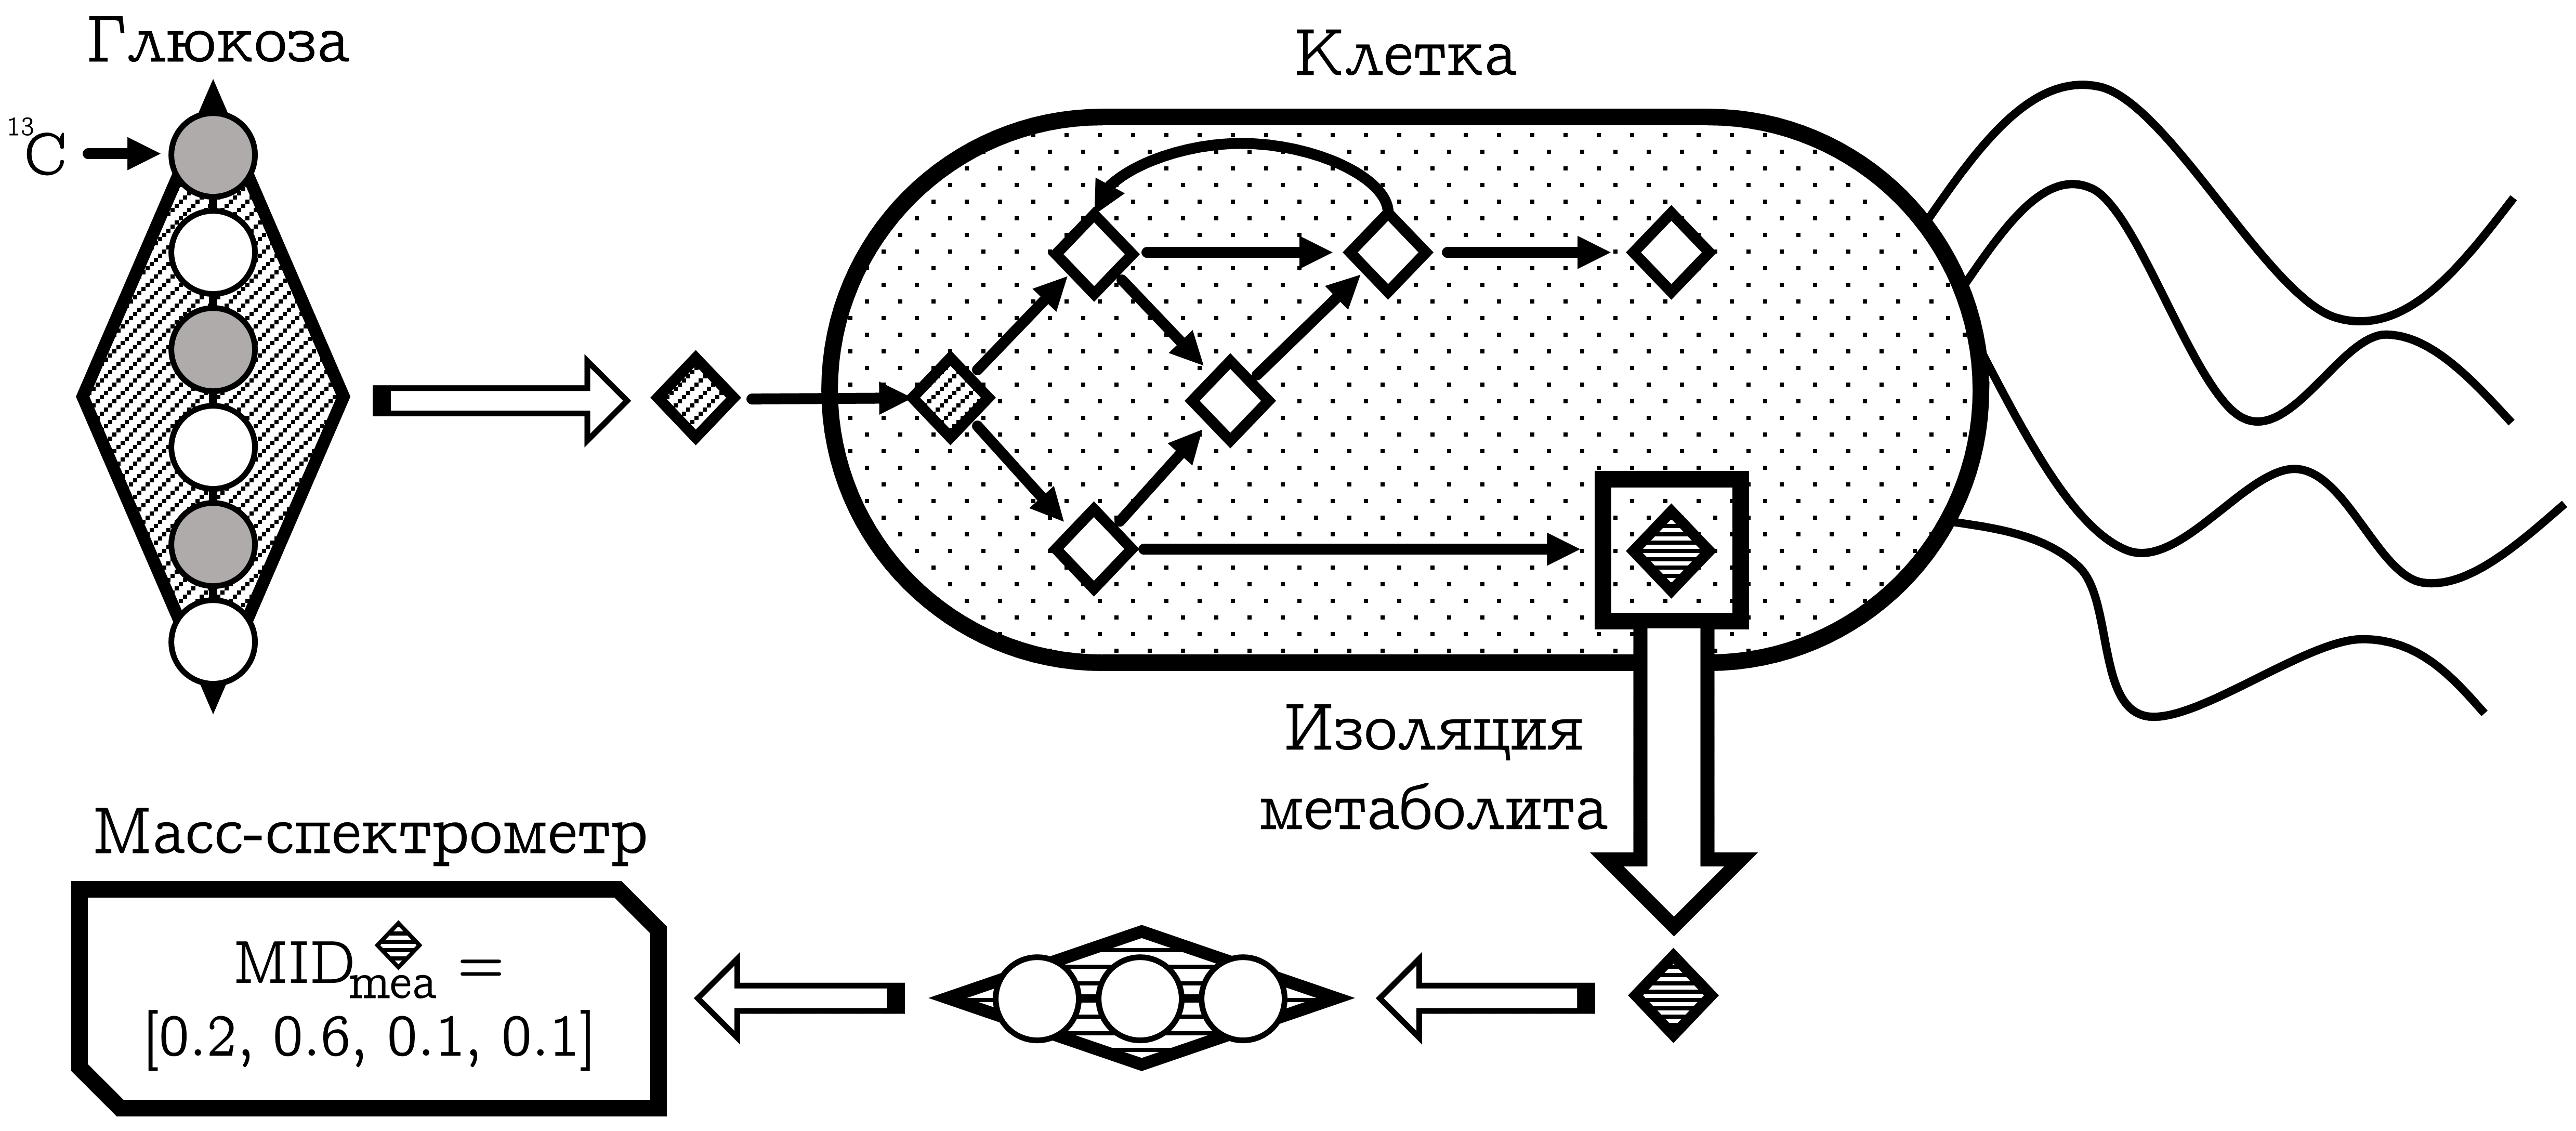
\includegraphics[width=1\textwidth]{experiment.png}\par
	\caption{Схема эксперимента}
	\label{experiment}
\end{figure}
Химические реакции, протекающие внутри клетки называют \emph{метаболическими потоками}, а их реагенты --- \emph{метаболитами}. Задача состоит в определении скоростей внутриклеточных потоков. 

Напрямую можно измерить только внешние потоки --- например, с какой скоростью поглощается глюкоза или с какой скоростью выделяется~\ce{CO_2}. Внутренние потоки восстанавливают из <<сцепленной>> информации, полученной в эксперименте. 

В методе \ce{^{13}C}-MFA <<сцепленной>> информацией становится распределение особых атомов. Для этого используется входной субстрат, у которого некоторые атомы углерода заменены на стабильный тяжелый изотоп \ce{^{13}C}, называемый \emph{трейсером}\footnote{На самом деле, использовать углерод не обязательно. В последнее время появились работы, использующие \ce{^{15}N} азот \cite{nitrogen_mfa} или \ce{^{34}S} серу \cite{sulfur_mfa}. Эти стабильные изотопы позволяют исследовать метаболические пути, в которых нет углерода, однако для большинства приложений хватает более доступных субстратов с меченным углеродом.}.
На этом субстрате выращивается колония клеток, и тяжелый углерод распространяется по метаболитам в ходе химических реакций. То, как он распределится, зависит от скоростей потоков, поэтому узнав распределение, можно математическими методами восстановить значения метаболических потоков.



\subsection{Эксперимент}
Хотя, текущая работа концентрируется на численном моделировании, опишем эксперимент\cite[стр. 312]{protocol}, схема которого изображена на рис. \ref{experiment}. Исследователь выращивает клетки на субстрате, содержащем \ce{^{13}C}-углерод (например, глюкозе). Когда трейсер распределится по биологической системе, изолируем некоторые метаболиты: например, аминокислоты, полученные гидролизацией белков. Молекулы этих метаболитов содержат разное количество меченных атомов и, поэтому отличаются по массе. Найдем долю молекул разной тяжести. 

<<Взвешивать>> молекулы можно с помощью газовой хромато-масс-\\спектрометрии, при этом для каждого метаболита на выходе получим так называемый \emph{Mass Isotopomer Distribution} (далее \emph{MID}) --- вектор $\boldsymbol{M\!I\!D} = [M_0, M_1, \ldots, M_n]$, где $M_i$ --- массовая доля метаболита с $i$ атомами трейсера, и $\sum_{i = 0}^{n} M_i= 1$ (См. таблицу \ref{MID}).

 \begin{wraptable}{r}{0.3\linewidth}
	\renewcommand{\arraystretch}{1.5}
	\begin{tabular}{c | c}
		\hline
		Меченность & Масса\\ 
		\hline
		
\includegraphics{emus/000.png} & $m_0$\\
		\hline
		
\includegraphics{emus/001.png} & \\
		
\includegraphics{emus/010.png} & $m_0 + 1$\\
		
\includegraphics{emus/100.png} & \\
		\hline
		
\includegraphics{emus/011.png} & \\
		
\includegraphics{emus/101.png} & $m_0 + 2$\\
		
\includegraphics{emus/110.png} & \\
		\hline
		
\includegraphics{emus/111.png} & $m_0 + 3$\\
	\end{tabular}
	\caption{Распределение трейсера и вес молекулы}
	\label{MID}
\end{wraptable} Набор таких векторов --- это распределение трейсера, 
 поэтому он служит входными данные математической задачи. Подробные протоколы эксперимента можно найти в \cite{protocol_animal} для животных клеток и в \cite{protocol_plant} для растений.


\subsection{Математическая модель}
Существуют разные подходы к вычислению метаболических потоков. Чаще всего задачу решают как обратную. Для этого создают математическую модель, предсказывающую MID метаболитов при заданных скоростях потока; пишут программу для симуляции, а затем решают задачу регрессии: подбирают такие значения потоков, при которых предсказанные в симуляции MID совпадают с полученными в эксперименте. 

На вход прямой симуляции подается 
\begin{itemize}
	\item MID входного субстрата.
	\item Полный набор химических реакций клетки и их реагентов.
	\item Скорости всех метаболических потоков.
\end{itemize}
На выходе получается MID-вектор экспериментально измеренных метаболитов. Общая схема представлена на рис. \ref{direct_simulation}.


На вход задачи регрессии также подаются MID входного субстрата и полный набор химических реакций, а кроме того:
\begin{itemize}
	\item Экспериментально измеренные MID некоторых метаболитов.
	\item Если есть --- измеренные внешние потоки (например, скорость поглощения глюкозы).
	\item Если есть --- ограничения на скорости потоков, известные из биологических соображений.
\end{itemize} 
В ходе решения регрессии, восстанавливаются скорости метаболических потоков. Конечно, обратная задача может иметь несколько решений, поэтому результат должен проанализироваться биологом. Формальное описание и решение модели в главе 2.

\clearpage
\begin{multicols}{2}[\subsubsection{Историческая справка}]
	\begin{table}[H]
		\renewcommand\arraystretch{1.4}
		\captionsetup{singlelinecheck=false, labelfont=sc, labelsep=quad}
		\caption{История}\vskip -1.5ex
		\begin{tabular}{@{\,}r <{\hskip 2pt} !{\foo} >{\raggedright\arraybackslash}p{5cm}}
			\toprule
			\addlinespace[1.5ex]
			1982 & Первый MFA с углеродом\cite{first_MFA}\\
			1988 & Появление термина <<изотопомер>>\\
			1997 & W. Weichert, изотопомерная модель\cite{Wiechert_1997_1, Wiechert_1997_2}\\
			1999 & W. Weichert, кумомерная модель\cite{Wiechert_1999_3, Wiechert_1999_4}\\
			2007 & W. Weichert, программа 13CFlux\cite{13CFlux1}\\
			2007 & M. Antoniewicz, EMU модель\cite{EMU_2007}\\
			2008 & M. Antoniewicz, программа Metran\cite{Metran}\\
			2009 & L. Quek, программа OpenFlux\cite{OpenFlux}\\
			2014 & М. Шуплецов, OpenFlux2\cite{OpenFlux2}\\
			2ххх & Еще какие-то программы\\
		\end{tabular}
	\end{table}
	\columnbreak
	
	\begin{figure}[H]
		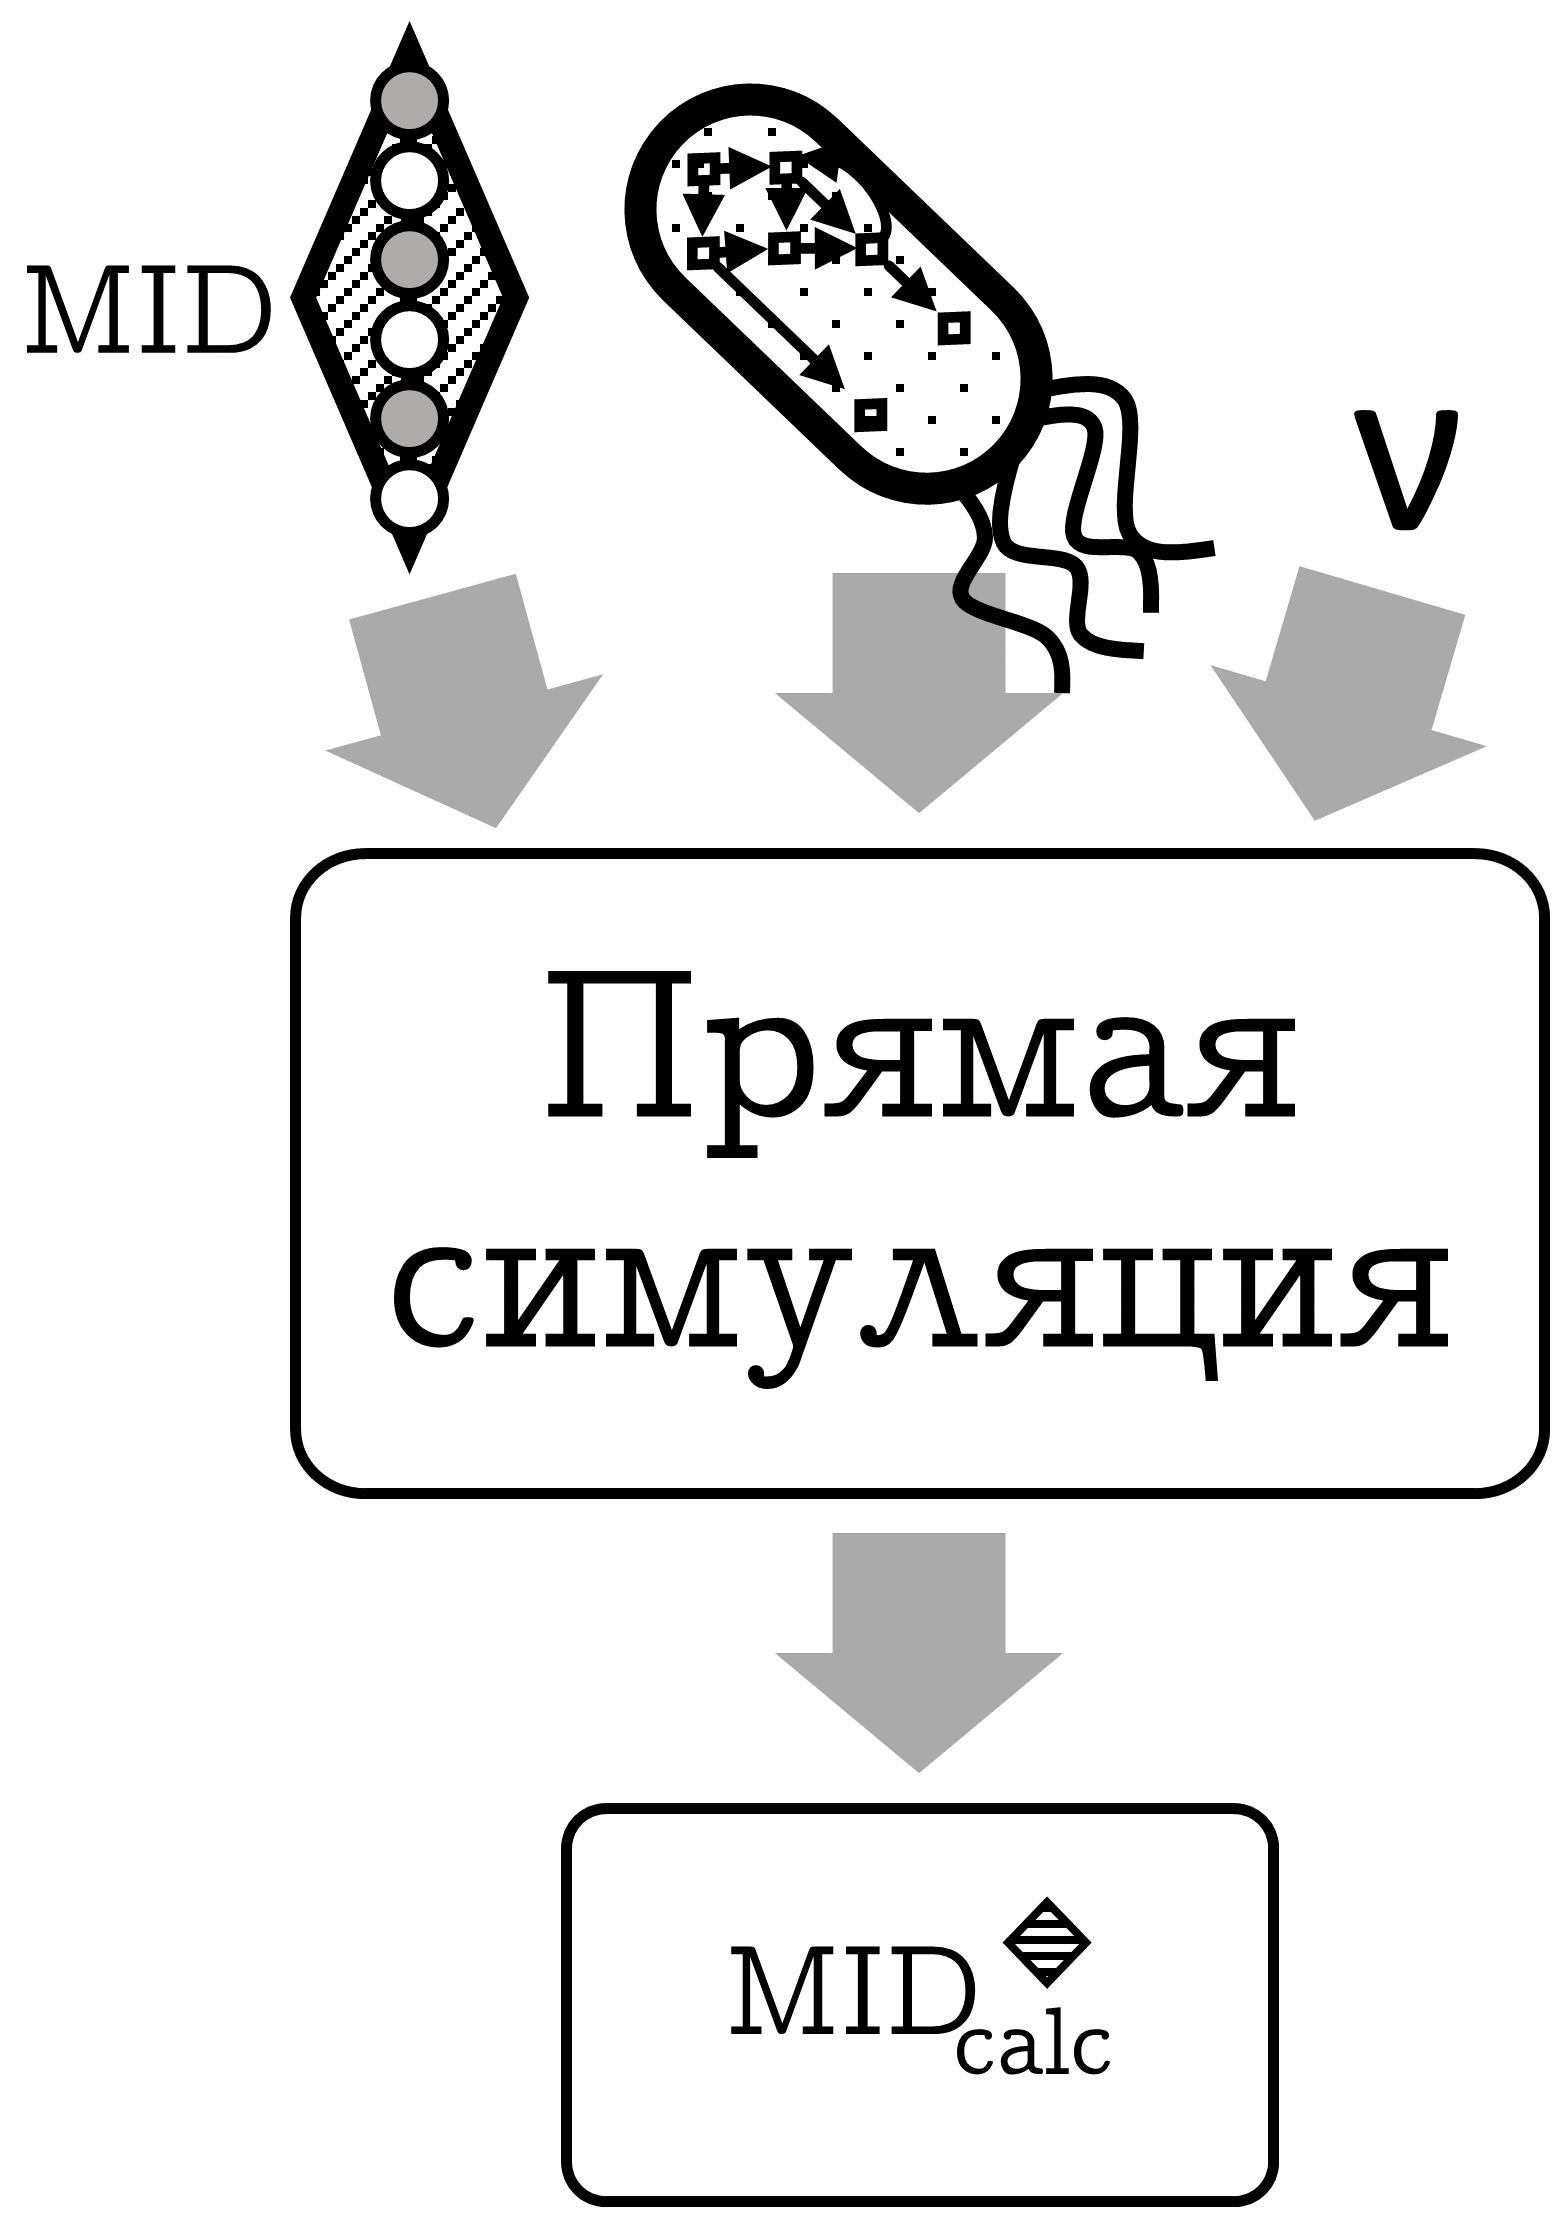
\includegraphics[width=0.9\linewidth]{direct_simulation.png}
		\captionof{figure}{Прямая симуляция}
		\label{direct_simulation}
	\end{figure}
	
	В восьмидесятые годы углерод начали использовать для анализа метаболических потоков. В 1997 году	
	W. Wiechert разработал удобную модель распространения углерода. Она использовала понятие \emph{изотопомера} --- это молекулы одного вещества, имеющие одинаковое количество атомов изотопов, вообще говоря в разных позициях. За два года автор разработал математически эквивалентную модель кумомеров, которая быстрее расчитывалась на компьютере. В 2007 году M. Antoniewicz создал EMU-модель, которая остается самой популярной среди программных реализаций. Так же существуют прямые модели\cite{Direct_MFA}, вероятностные модели на основе Марковских цепей\cite{Markov_chain_MFA} и другие\cite{Fluxomer_MFA}. В этой работе подробно разбирается EMU-модель.
\end{multicols}



\begin{comment}

\sidebyside[0.4][0.6]{
	\begin{minipage}{\linewidth}
		\begin{table}[H]
			\renewcommand\arraystretch{1.4}
			\captionsetup{singlelinecheck=false, labelfont=sc, labelsep=quad}
			\caption{История}\vskip -1.5ex
			\begin{tabular}{@{\,}r <{\hskip 2pt} !{\foo} >{\raggedright\arraybackslash}p{4cm}}
				\toprule
				\addlinespace[1.5ex]
				1982 & Первый MFA с углеродом\cite{first_MFA}\\
				1988 & Появление термина <<изотопомер>>\\
				1997 & W. Weichert, изотопомерная модель\cite{Wiechert_1997_1, Wiechert_1997_2}\\
				1999 & W. Weichert, кумомерная модель\cite{Wiechert_1999_3, Wiechert_1999_4}\\
				2007 & M. Antoniewicz, EMU модель\cite{EMU_2007}\\
				2007 & M. Antoniewicz, EMU модель\cite{EMU_2007}\\
				2007 & M. Antoniewicz, EMU модель\cite{EMU_2007}\\
				2007 & M. Antoniewicz, EMU модель\cite{EMU_2007}\\
				2007 & M. Antoniewicz, EMU модель\cite{EMU_2007}\\
				2007 & M. Antoniewicz, EMU модель\cite{EMU_2007}\\
				2007 & M. Antoniewicz, EMU модель\cite{EMU_2007}\\
			\end{tabular}
		\end{table}
	\end{minipage}
}{\noindent
		рукру
		\begin{figure}[H]
			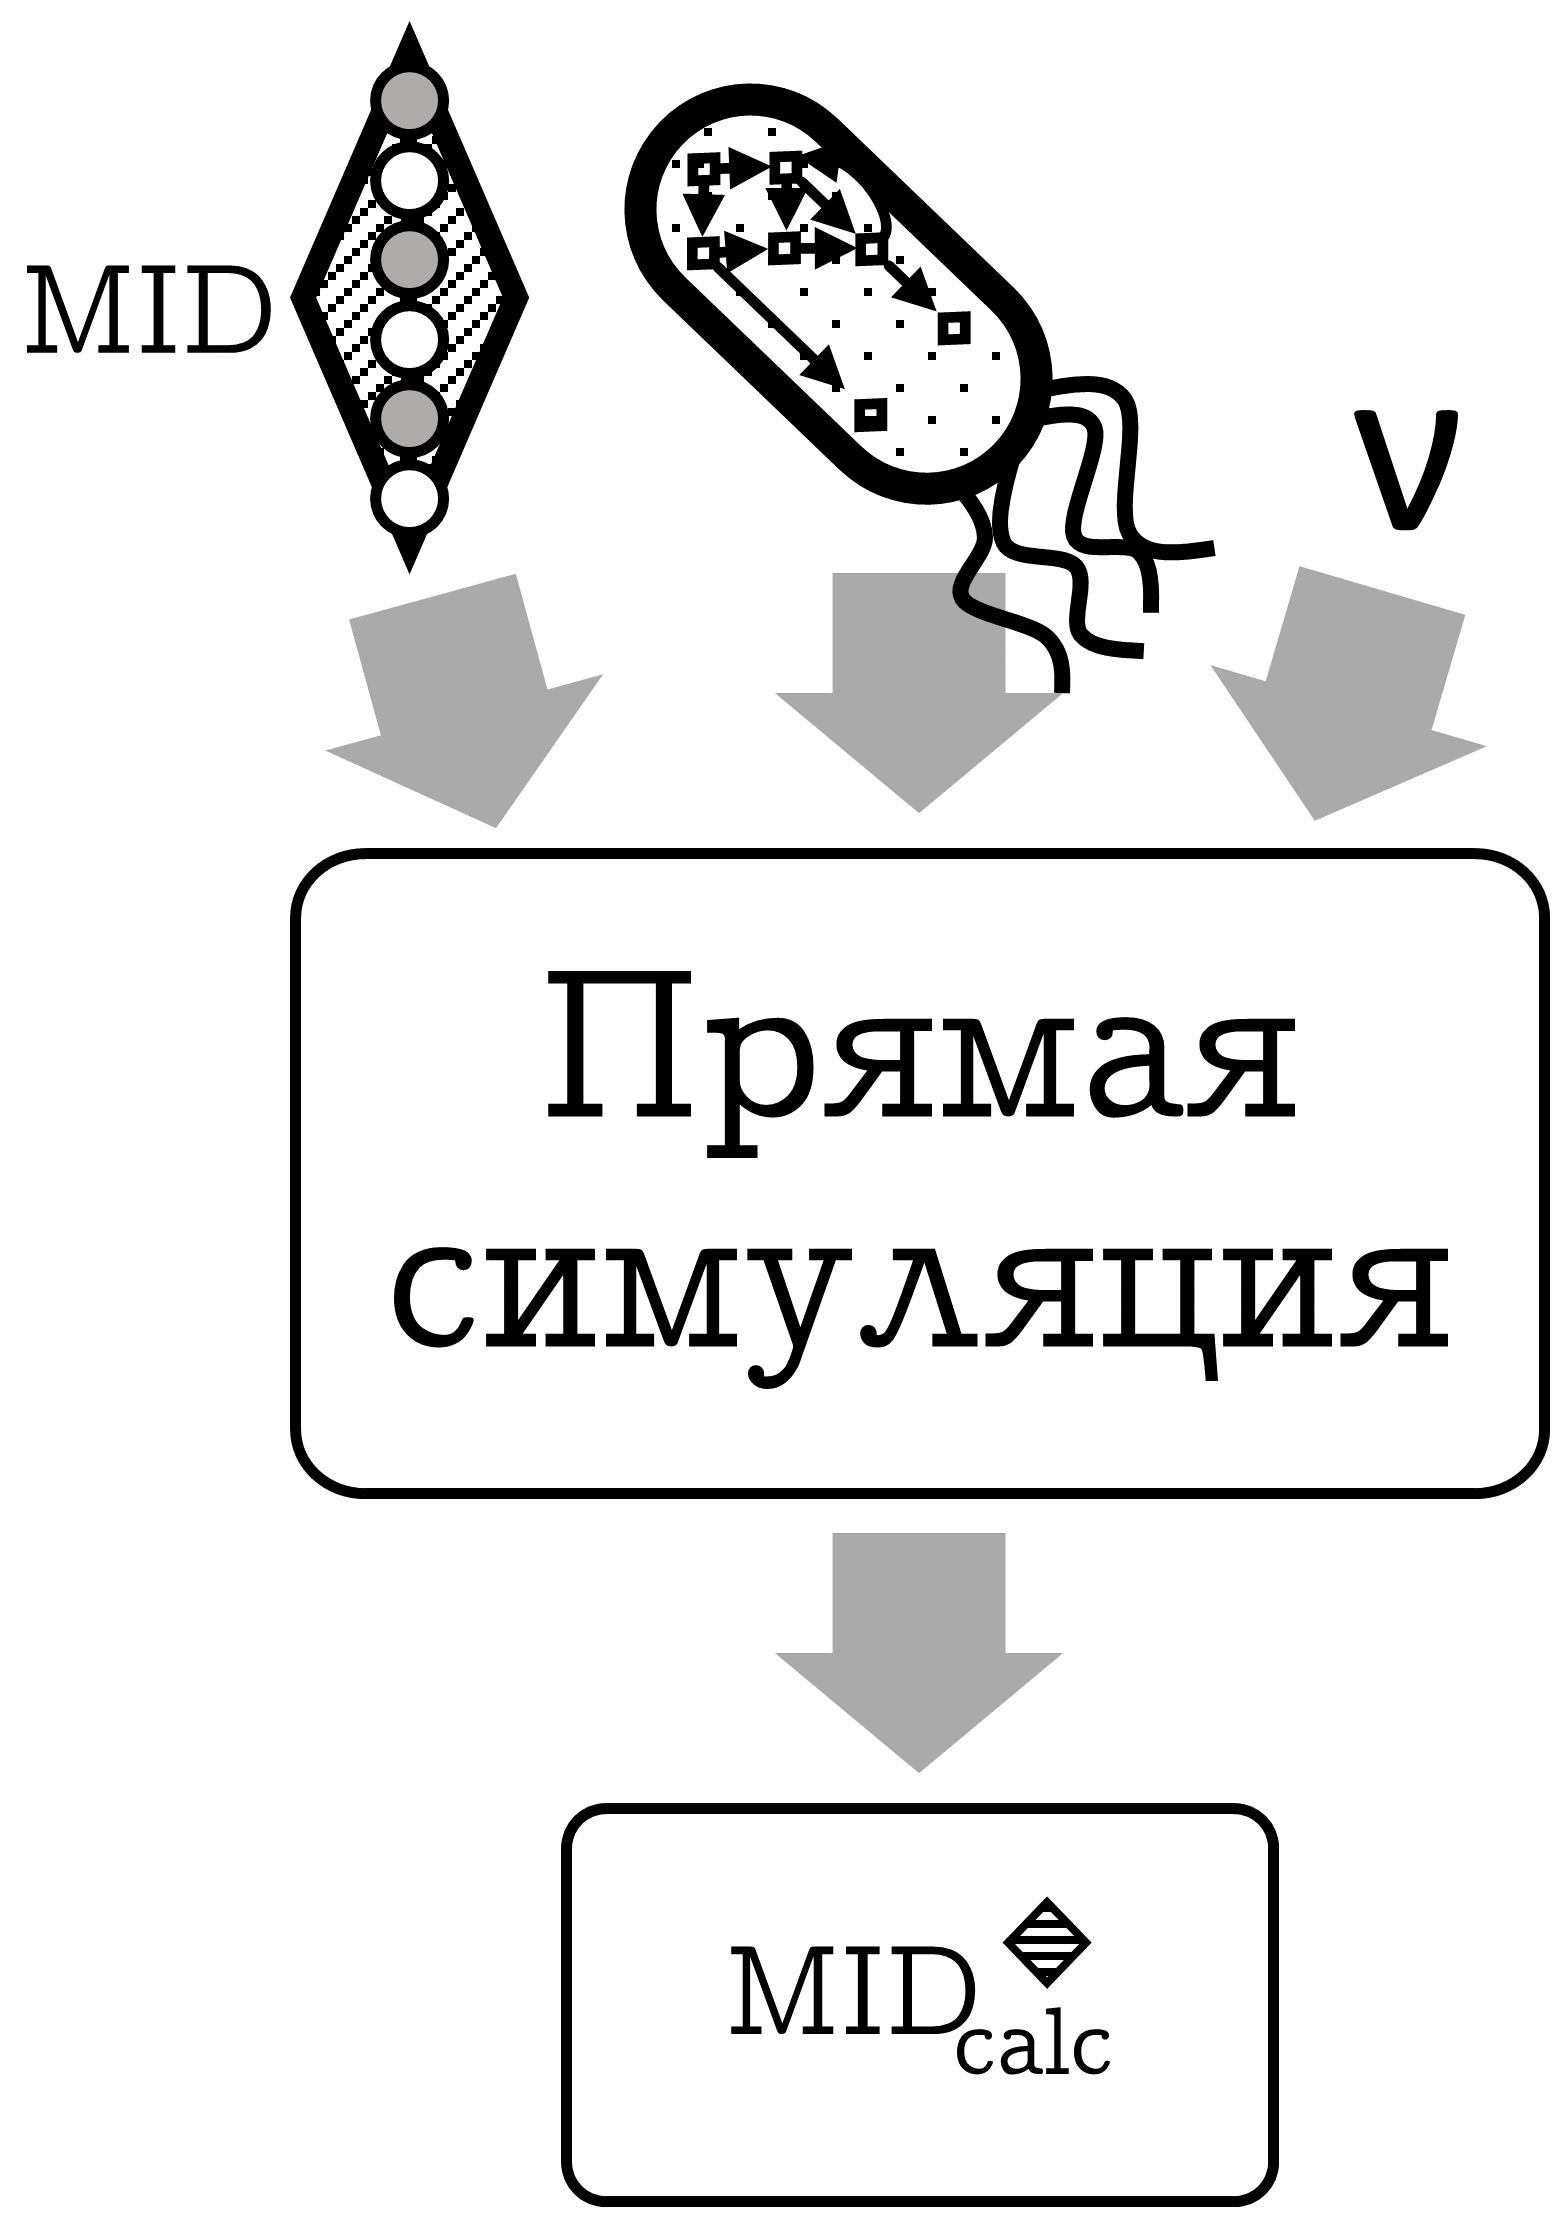
\includegraphics[width=1\linewidth]{direct_simulation.png}
			\captionof{figure}{Прямая симуляция}
			\label{direct_simulation}
		\end{figure}
	
		В восьмидесятые годы углерод начали использовать для анализа метаболических потоков. В 1997 году	
		W. Wiechert разработал удобную модель распространения углерода. Она использовала понятие \emph{изотопомера} --- это молекулы одного вещества, имеющие одинаковое количество атомов изотопов, вообще говоря в разных позициях. За два года автор разработал математически эквивалентную модель кумомеров, которая быстрее расчитывалась на компьютере. В 2007 году M. Antoniewicz создал EMU-модель, которая остается самой популярной среди программных реализаций. Так же существуют прямые модели\cite{Direct_MFA}, вероятностные модели на основе Марковских цепей\cite{Markov_chain_MFA} и другие\cite{Fluxomer_MFA}. В этой работе подробно разбирается EMU-модель.
}
content...
\end{comment}




%\begin{wraptable}[20]{l}{0.4\linewidth}
	
%\end{wraptable}






\clearpage
\subsection{Компьютерные программы}
Существует несколько программ для \ce{^{13}C}-MFA расчетов (См. приложение А). 
План: провести замеры -> дописать список программ -> дописать этот раздел.

\chapter[Основные понятия]{\thechapter{}. Основные понятия}
\section{Список определений}
Некоторые термины вводятся позже.

\hangindent=1cm \noindent
\emph{\ce{^{13}C}-MFA} --- \ce{^{13}C}-Metabolic Flux Analysis, Анализ метаболических потоков с использованием \ce{^{13}C}-углерода.

\hangindent=1cm \noindent
\emph{Метаболический поток} --- Внутриклеточная химическая реакция.

\hangindent=1cm \noindent
\emph{Метаболит} --- Реагент метаболического потока.

\hangindent=1cm \noindent
\emph{Субстрат} --- 1. Питательная среда для микроорганизмов. 2. Исходные реагенты химической реакции.

\hangindent=1cm \noindent
\emph{Продукт} --- Конечные реагенты химической реакции.

\hangindent=1cm \noindent
\emph{Трейсер} --- Тяжелый стабильный изотоп, который отслеживается в MFA. Обычно это \ce{^{13}C}.

\hangindent=1cm \noindent
\emph{MID} --- Mass Isotope Distribution, вектор $\boldsymbol{M\!I\!D} = [M_0, M_1, \ldots, M_n]$, соответствующим метаболиту $M$, где $M_i$ --- массовая доля молекул метаболита с $i$ атомами трейсера, и $\sum_{i = 0}^{n} M_i = 1$.

\hangindent=1cm \noindent
\emph{Изотопомеры} --- Молекулы одного вещества, содержащие одинаковое количество изотопов и, как следствие, массу. Изотопы могут находится в разных позициях.

\hangindent=1cm \noindent
\emph{Стехиометрическая матрица} --- Матрица $\boldsymbol{S}$, в которой каждый элемент $s_{ij}$ равен коэффициенту метаболита $M_i$ в химическом уравнении $K_j$. В стационарной системе, при умножении на столбец метаболических потоков даст ноль.

\hangindent=1cm \noindent
\emph{Метаболическая сеть} --- Ориентированный гиперграф, вершины которого --- метаболиты, ребра --- химические реакции, и для каждой химической реакции известно, какой атом трейсера в какой переходит.\footnote{Формальное определение в приложении Б.}

\hangindent=1cm \noindent
\emph{EMU} --- Elementary Metabolic Unit молекулы --- это любое непустое подмножество атомов трейсера этой молекулы.

\hangindent=1cm \noindent
\emph{Размер EMU} --- Количество атомов в EMU.

\hangindent=1cm \noindent
\emph{Размер EMU-реакции} --- Сумма размеров реагентов EMU-реакции.

\hangindent=1cm \noindent
\emph{EMU-граф} --- граф EMU-реакций одного размера.



\clearpage

\section{Предположения}
Математическая модель для \ce{^{13}C}-MFA основывается на нескольких предположениях о биологической системе\cite{Wiechert_1997_1}:
\begin{enumerate}
	\item[(1П)] Наблюдаемая система должна находится в стационарном состоянии. Для этого экспериментаторы выжидают некоторое время, пока трейсер распространяется по системе.\footnote{В этой работе рассматривается только \emph{Stationary MFA}, но существуют так же Non-Steady MFA\cite{NMFA}, в котором делают несколько замеров, пока трейсер распределяется, и Dynamic MFA\cite{DMFA}, в котором сами метаболические потоки меняются со временем. Эти модели не так развиты из-за своей вычислительной сложности.}
	
	\item[(2П)] Метаболическая карта должна быть полной. То есть, для интересующих метаболических потоков должны быть известны все предшествующие химические реакции, и в них должны быть известны все переходы атомов углерода.
	
	\item[(3П)] Изотопические массовые эффекты несущественны. То есть химические реакции протекают одинаково как с \ce{^{12}C}, так и с \ce{^{13}C}. Это обычно так, но есть небольшие отличия для малых молекул, например, \ce{CO_2}.
	
	\item[(4П)] Популяция клеток однородна. Современные техники позволяют измерять потоки <<в среднем>>. Это сработает только, если клетки не сильно отличаются друг от друга.
\end{enumerate}

Заметим, что разным математическим моделям могут соответствовать разные допущения. Этот вопрос подробно разбирался в работе \cite{formalizm_2017}, там же формально был доказан изоморфизм нескольких популярных моделей.
\clearpage


\section{Обратная задача}

Сформулируем обратную задачу как задачу минимизации. Пусть $\boldsymbol{v}$ --- скорости метаболических потоков. На потоки накладываются разные ограничения, поэтому они должны принадлежать \emph{пространству допустимых потоков} $U \subset \mathbb{R}^n$. Подберем такие $\boldsymbol{v} \in U$, чтобы минимизировать квадрат разности между экспериментально измеренными MID метаболитов $\boldsymbol{x}_{mea}$ и предсказанными\footnote{Предсказанию $\boldsymbol{x}_{calc}(\boldsymbol{v})$ посвящен следующий раздел 2.4 Прямая симуляция.} MID метаболитов $\boldsymbol{x}_{calc}(\boldsymbol{v})$. Для этого учтем, что измерения проводились с погрешностью. 

Пусть $\boldsymbol{\sigma}_{mea}$ --- ошибки измерения $\boldsymbol{x}_{mea}$, $\boldsymbol{\Sigma}(\boldsymbol{\sigma}_{mea})$ --- матрица ковариации ошибок измерения. Если ошибки независимы, распределены нормально и нескоррелированны, то $\boldsymbol{\Sigma}(\boldsymbol{\sigma}_{mea})$ --- это диагональная матрица \\$diag(\sigma_{1}^2, \sigma_{2}^{2}, \dots, \sigma_{n}^2)$. Тогда математическая задача \ce{{}^13C}-MFA формулируется так:
$$\min_{\boldsymbol{v} \in U}{ } (\boldsymbol{x}_{mea} - \boldsymbol{x}_{calc}(\boldsymbol{v}))^T \times \boldsymbol{\Sigma}^{-1} \times (\boldsymbol{x}_{mea} - \boldsymbol{x}_{calc}(\boldsymbol{v})) \eqno (1.1)$$


\begin{wrapfigure}{r}{0.5\linewidth}
	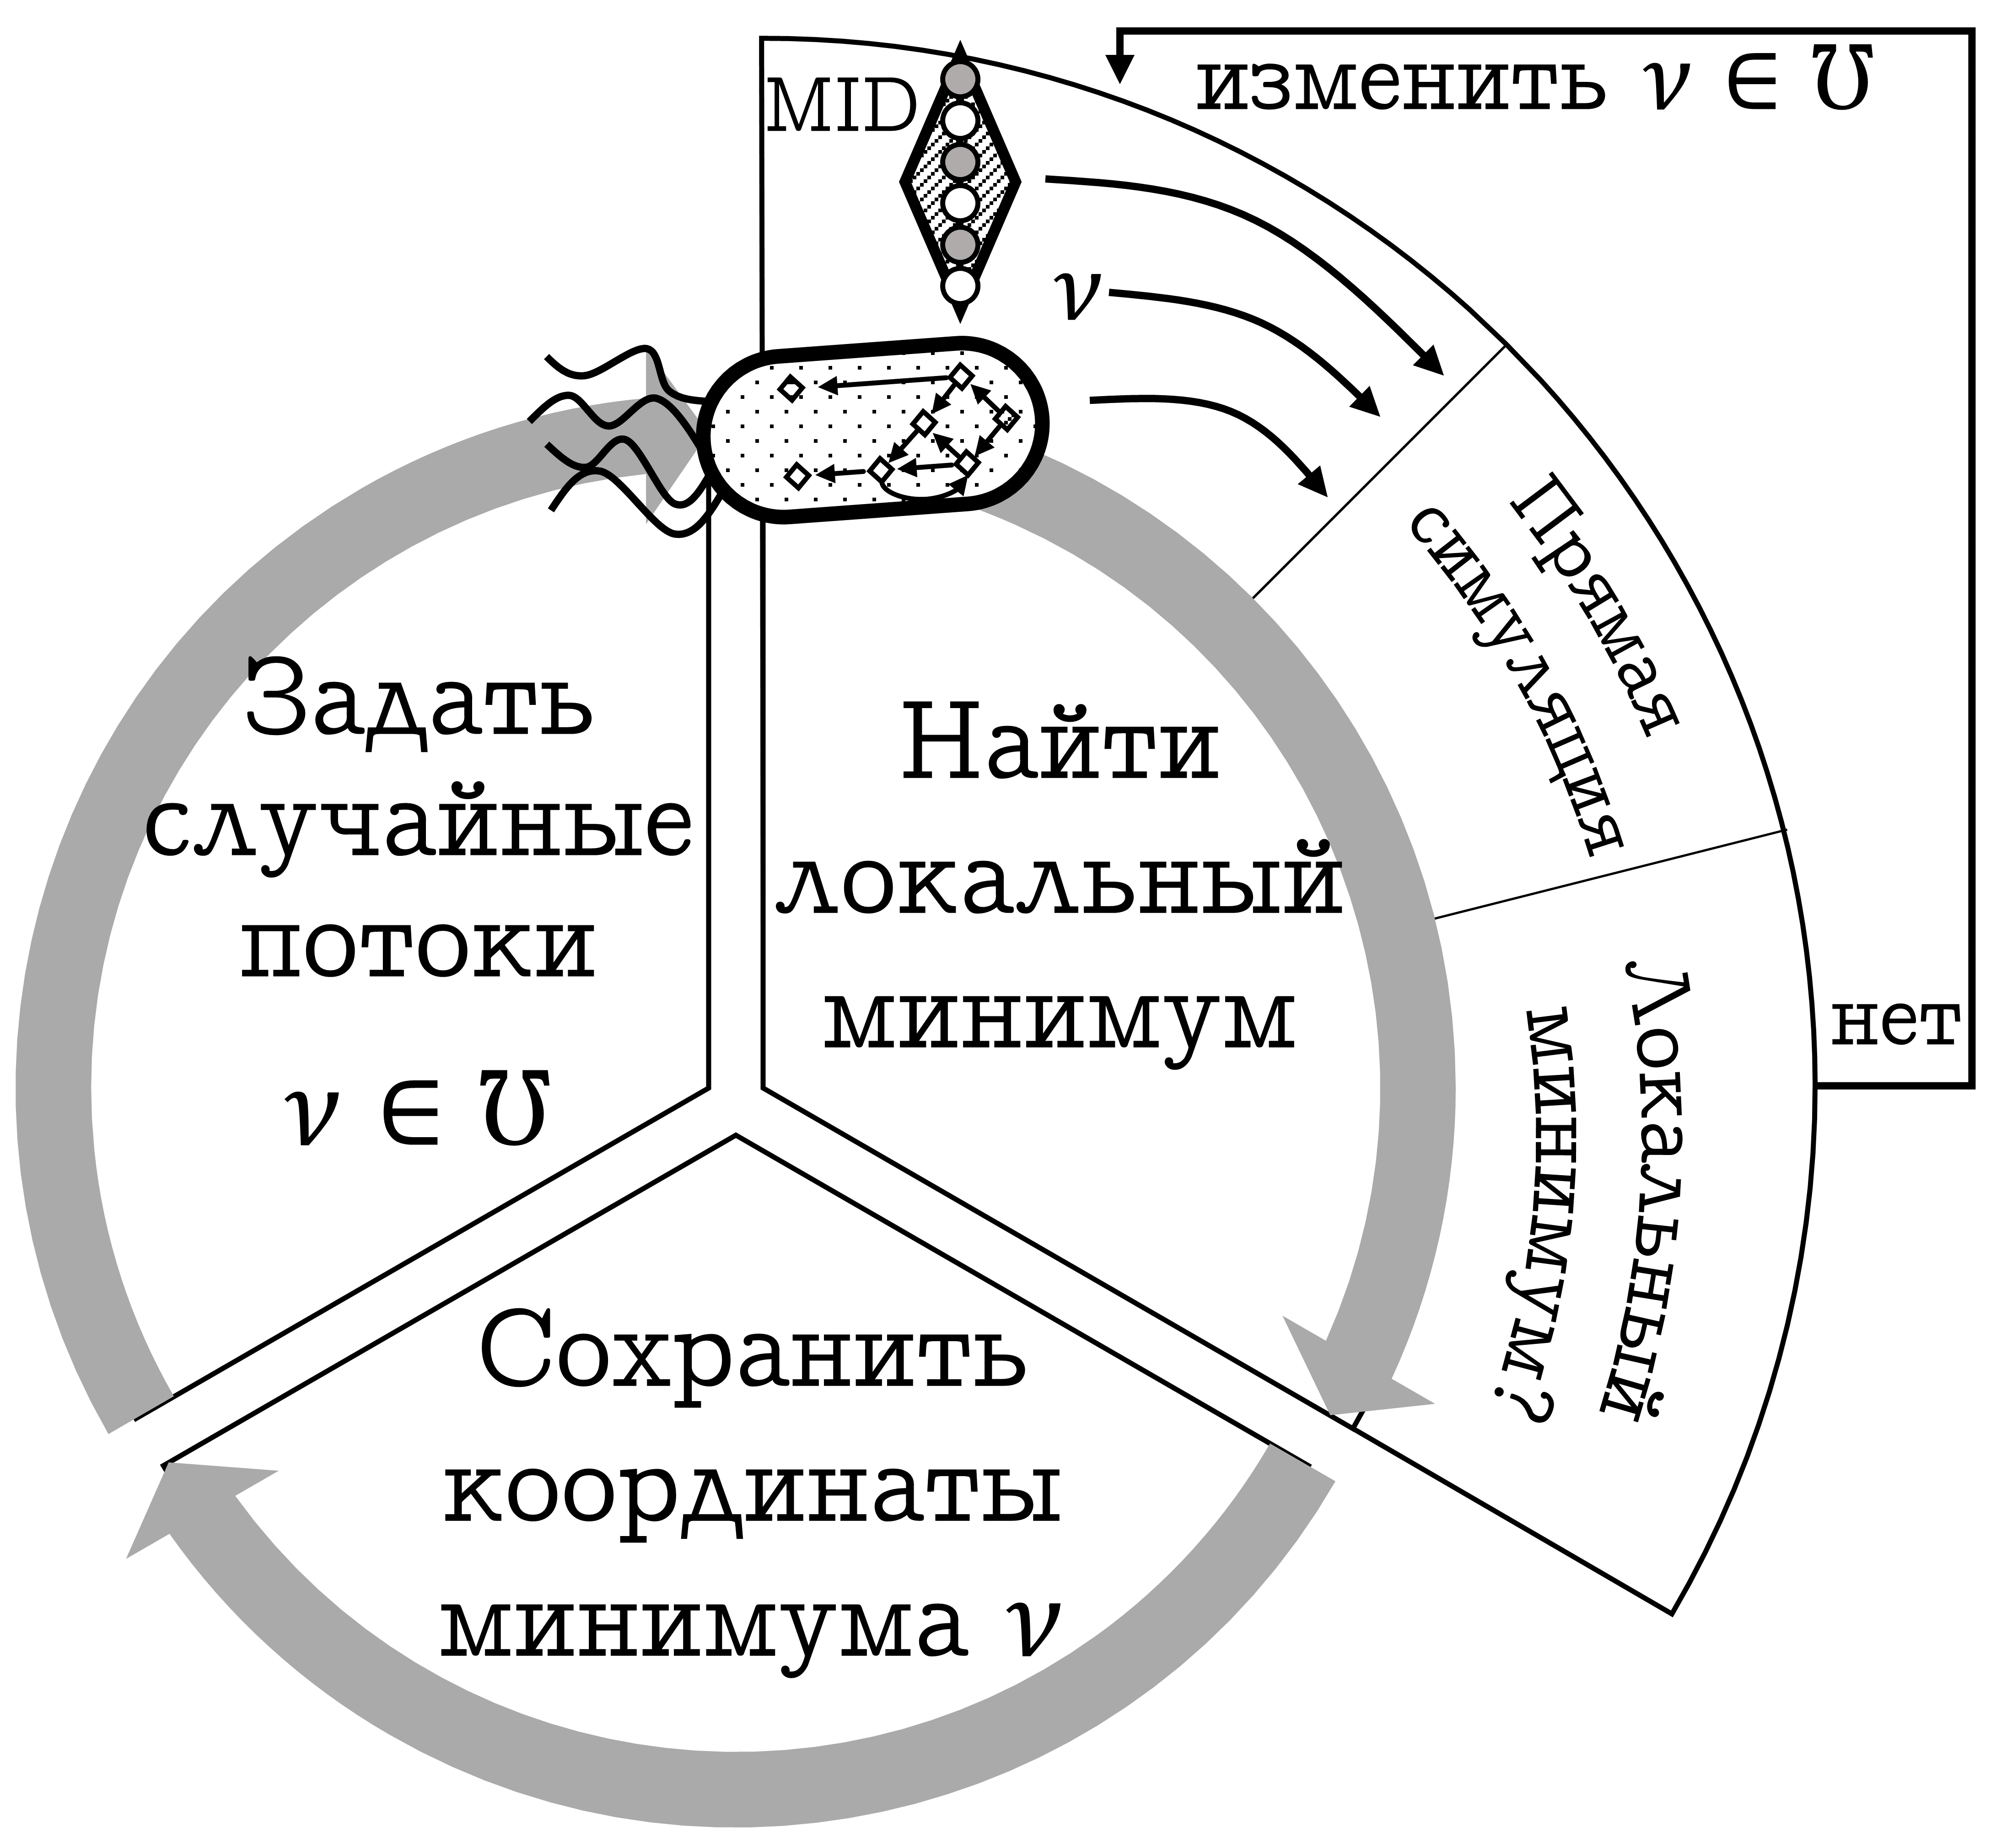
\includegraphics[width=1\linewidth]{inverse_problem.png}
	\captionof{figure}{Обратная задача}
	\label{inverse_problem}
\end{wrapfigure}

Существуют различные оптимизационные методы решения этой задачи. Чаще всего применяется метод Монте-Карло вместе с градиентным спуском (см. рис \ref{inverse_problem}). Для этого начальные потоки $\boldsymbol{v} \in U$ задаются случайно, и запускается метод оптимизации, который учитывает ограничения $U$. Когда минимум найден, его координаты сохраняются и процесс запускается снова. Через достаточное количество итераций, мы можем получить несколько глобальных минимумов, один из которых соотвествует искомым метаболическим потокам $\boldsymbol{v}$. Его выбирают из биологических соображений.

Обсудим пространство допустимых потоков $U$. Чем оно меньше, тем быстрее найдется глобальный минимум. Для каждого потока можно считать, что он неотрицателен и ограничен сверху. Биолог может задать дополнительные ограничения --- в большинстве случаев, линейные. Кроме того, мы можем уменьшить размерность системы.

\subsection{Стехиометрическая матрица}

Введем понятие \emph{стехиометрической матрицы}. Пусть $M_1, M_2, \dots, M_n$ --- метаболиты, $K_1, K_2, \dots, K_m$ --- система химических уравнений. 
Составим матрицу $\boldsymbol{S} \in \mathbb{R}^{n \times m}$ порядка $n \times m$. В ней элемент $s_{ij}$ равен коэффициенту метаболита $M_i$ в уравнении $K_j$.

Например, рассмотрим химическое уравнение:

\begin{center}
	\ce{Na + H_2O = NaOH + H_2}
\end{center}

Расставим коэффициенты:

\begin{center}
	\ce{2Na + 2H_2O = 2NaOH + H_2}
\end{center}

Перенесем все в левую часть:

\begin{center}
	\ce{2Na + 2H_2O - 2NaOH - H_2 = 0}
\end{center}
Тогда этому уравнению будет соответствовать столбец $\begin{pmatrix}
2 & 2 & -2 & -1\\
\end{pmatrix}^T$. Сделав так для каждого уравнения системы, получим разреженную матрицу, которую называют \emph{стехиометрической}.

Запишем, так называемое, уравнение материального баланса:

$$\frac{d\textbf{c}}{dt} = \textbf{Sv} - \mu{}\textbf{c}$$

Здесь записан закон сохранения массы в дифференциальном виде. $\textbf{c}$~---~столбец концентраций метаболитов, $\textbf{S}$ --- стехиометрическая матрица, $\textbf{v}$ --- столбец метаболических потоков. Коэффициент $\mu$ отвечает за разведение метаболитов из-за клеточного роста, со скоростью $\mu$. По предположению (1П), система находится в стационарном состоянии, поэтому концентрации метаболитов не меняются $\frac{d\textbf{c}}{dt} = 0$. Клетки растут медленно, коэффициент $\mu$ обычно мал и им можно пренебречь. Тогда:
$$ \textbf{Sv} = 0$$
Обычно, $\boldsymbol{S}$ --- неполного ранга, поэтому систему можно параметризовать:
$$ \boldsymbol{v} = ker(\boldsymbol{S}) \cdot \boldsymbol{v}_{free}$$
где $ker(\textbf{S})$ --- матрица ядра стехиометрической матрицы $\boldsymbol{S}$. Ее подбирают таким образом, чтобы в $\boldsymbol{v}_{free}$ было как можно больше экспериментально измеренных внешних потоков.

Кроме параметризации, такое условие $\boldsymbol{v} = ker(\boldsymbol{S}) \cdot \boldsymbol{v}_{free}$ позволяет сузить пространство допустимых потоков $U$ линейными ограничениями, если учесть, что потоки ограничены: $\boldsymbol{0} \le \boldsymbol{v} = ker(\boldsymbol{S}) \cdot \boldsymbol{v}_{free} \le \boldsymbol{b}$.



\clearpage
\section{Прямая симуляция}
Опишем модель EMU, предложенную Мачеком Антониевичем в 2007 году\cite{EMU_2007}. Рассмотрим ориентированный гиперграф, вершины которого соответствуют метаболитам, а ребра --- химическим реакциям. Для каждой реакции известно какой атом углерода в какой переходит. Такой граф называют \emph{метаболической сетью}\footnote{Пример на рис. \ref{emu_example}. Формальное определение не вносит ясности и вынесено в приложение~Б.}. 

На вход прямой симуляции подается:
\begin{itemize}
	\item MID входных субстратов.
	\item Метаболическая сеть.
	\item Скорости всех потоков.
\end{itemize}
На выходе --- MID экспериментально измеренных метаболитов.
Для этого мы построим графы специального вида (\emph{графы EMU-реакций}), по которым построим каскад СЛАУ, решение которых содержит искомые MID.
\subsection{EMU}

\begin{wraptable}{r}{0.35\linewidth}
	\begin{tabular}{c | c}
		EMU & Обозначение\\
		\hline
		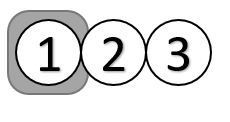
\includegraphics[scale=0.6]{emus/EMUA1.png} & $A_1$\\
		\hline
		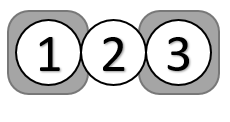
\includegraphics[scale=0.6]{emus/EMU13.png} & $A_{13}$\\
		\hline
		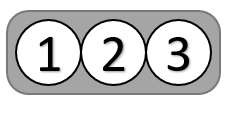
\includegraphics[scale=0.6]{emus/EMU123.png} & $A_{123}$\\
	\end{tabular}
	\caption{Обозначения EMU}
	\label{EMU}
\end{wraptable}

Пусть $A$ --- молекула. Любое подмножество атомов трейсера молекулы $A$ будем называть \emph{Elementary Metabolic Unit} (далее \emph{EMU}). Например, если $A$ состоит из трех атомов трейсера, обозначим через $A_{13}$ EMU состоящее из первого и третьего атома углерода (см. рис \ref{EMU}). На атомах трейсера одной молекулы задан естественный порядок. \emph{Размером} EMU назовем количество атомов в этом EMU.

Нас интересует только распределение трейсера, поэтому вместо всех метаболитов сети, будем рассматривать только их EMU. Вместо химических реакций, будем рассматривать EMU-реакции. Можно выделить три типа EMU-реакций (см. таблицу \ref{EMU_reactions}):
\begin{itemize}
	\item Конденсации (condensation)
	\item Расщепления (cleavage)
	\item Унимолекулярная (unimolecular)
\end{itemize}
Любую химическую реакцию можно свести к нескольким EMU-реакциям этих типов. Обратим внимание, что MID продукта EMU-реакции однозначно определяется MID исходных субстратов. С этого момента будем ассоциировать обозначение EMU с его MID.
\clearpage

\begin{table}
	\begin{center}
		\begin{tabular}{c | c}
			\hline
			EMU-реакция & MID\\
			\hline
			\multirow{5}{*}[-1mm]{
				\begin{minipage}{0.3\linewidth}
					\centering{Реакция конденсации}
					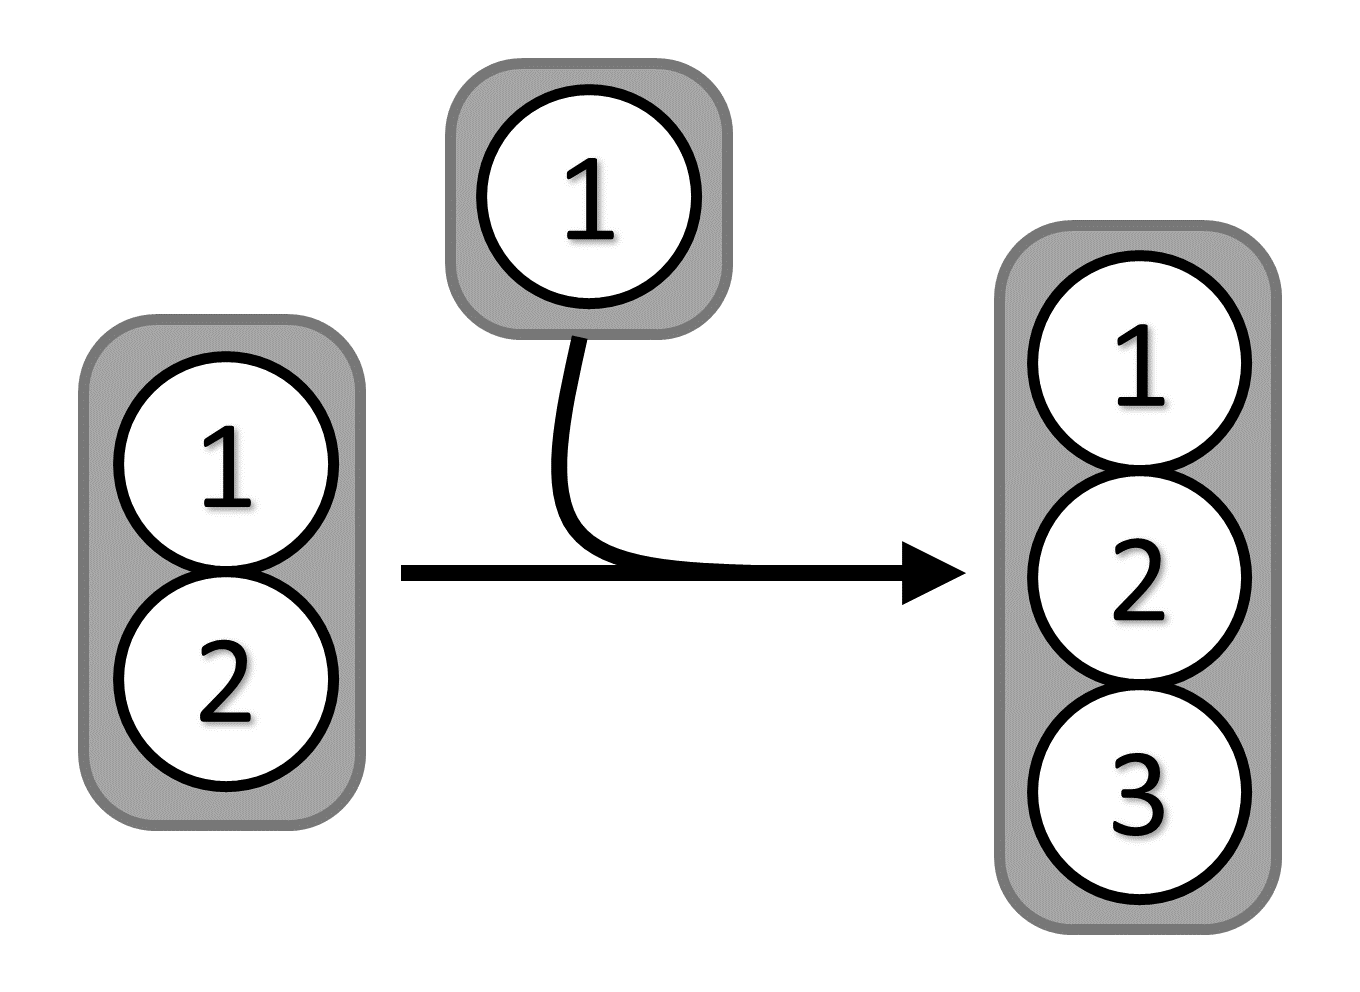
\includegraphics[scale=0.85]{EMU_reaction_1.png}
				\end{minipage}
			} 
			  & \adj{$C_{123} = A_{12} \times B_1$}\\[0.5ex]
			  & \adj{$C_{123,M+0} = A_{12,M+0} \cdot B_{1,M+0}$}\\ [0.5ex]
			  & \adj{$C_{123,M+1} = A_{12,M+0} \cdot B_{1,M+1} + A_{12,M+1} \cdot B_{1,M+0}$}\\ [0.5ex]
			  & \adj{$C_{123,M+2} = A_{12,M+1} \cdot B_{1,M+1} + A_{12,M+2} \cdot B_{1,M+0}$}\\ [0.5ex]
			  & \adj{$C_{123,M+3} = A_{12,M+2} \cdot B_{1,M+1}$} \\ [0.5ex]
			 \hline 
			 \multirow{5}{*}[-1mm]{
			 	\begin{minipage}{0.3\linewidth}
			 		\centering{Реакция расщепления}
			 		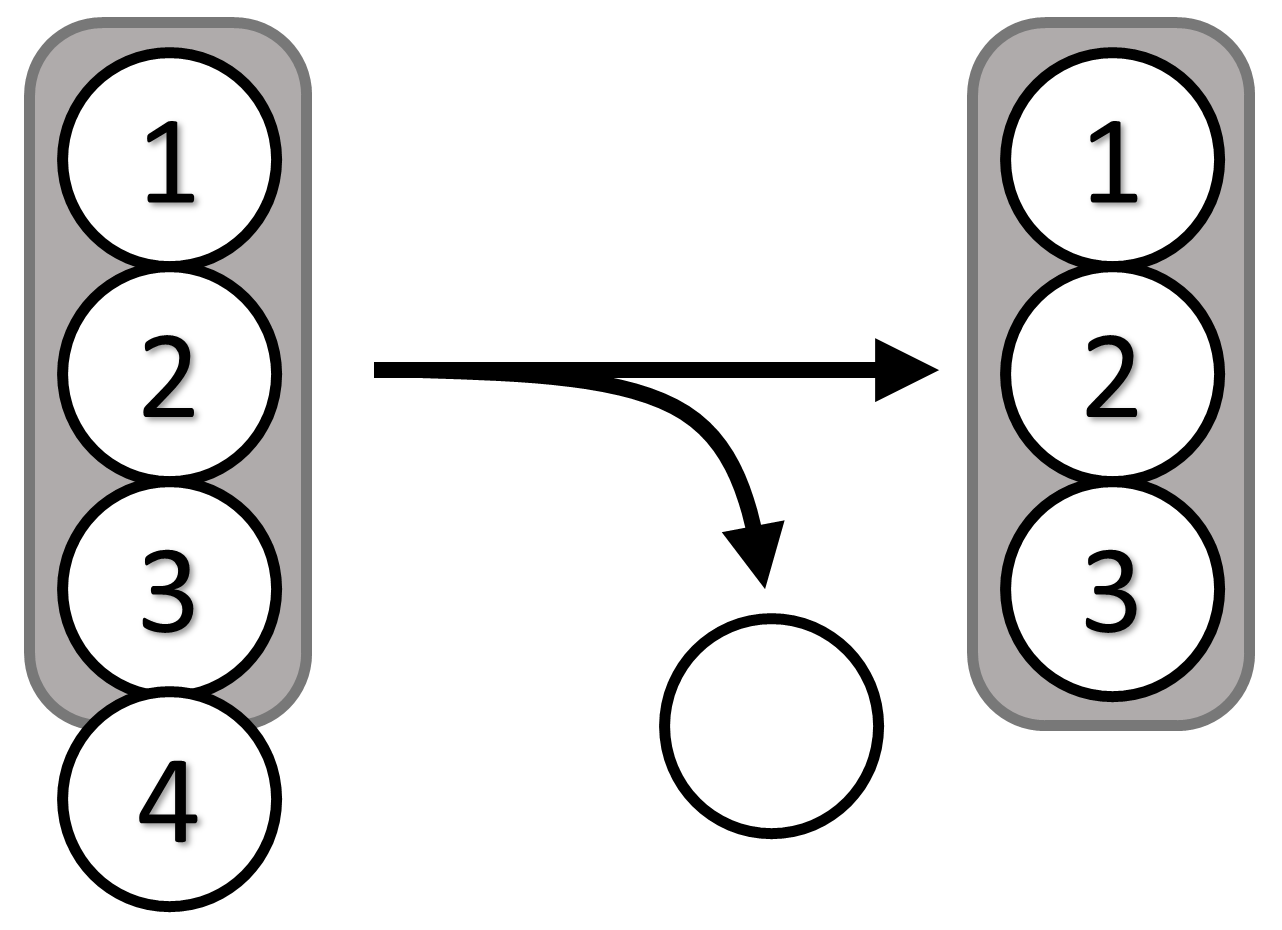
\includegraphics[scale=0.85]{EMU_reaction_2.png}
			 	\end{minipage}
			 } 
		     & \adj{$C_{123} = A_{123}$}\\[.5ex]
			 & \adj{$C_{123,M+0} = A_{123,M+0}$}\\ [.5ex]
			 & \adj{$C_{123,M+1} = A_{123,M+1}$}\\ [.5ex]
			 & \adj{$C_{123,M+2} = A_{123,M+2}$} \\ [.5ex]
			 & \adj{$C_{123,M+3} = A_{123,M+3}$} \\ [.5ex]
			 \hline 
			 \multirow{5}{*}[-1mm]{
			 	\begin{minipage}{0.3\linewidth}
			 		\centering{Унимолекулярная реакция}
			 		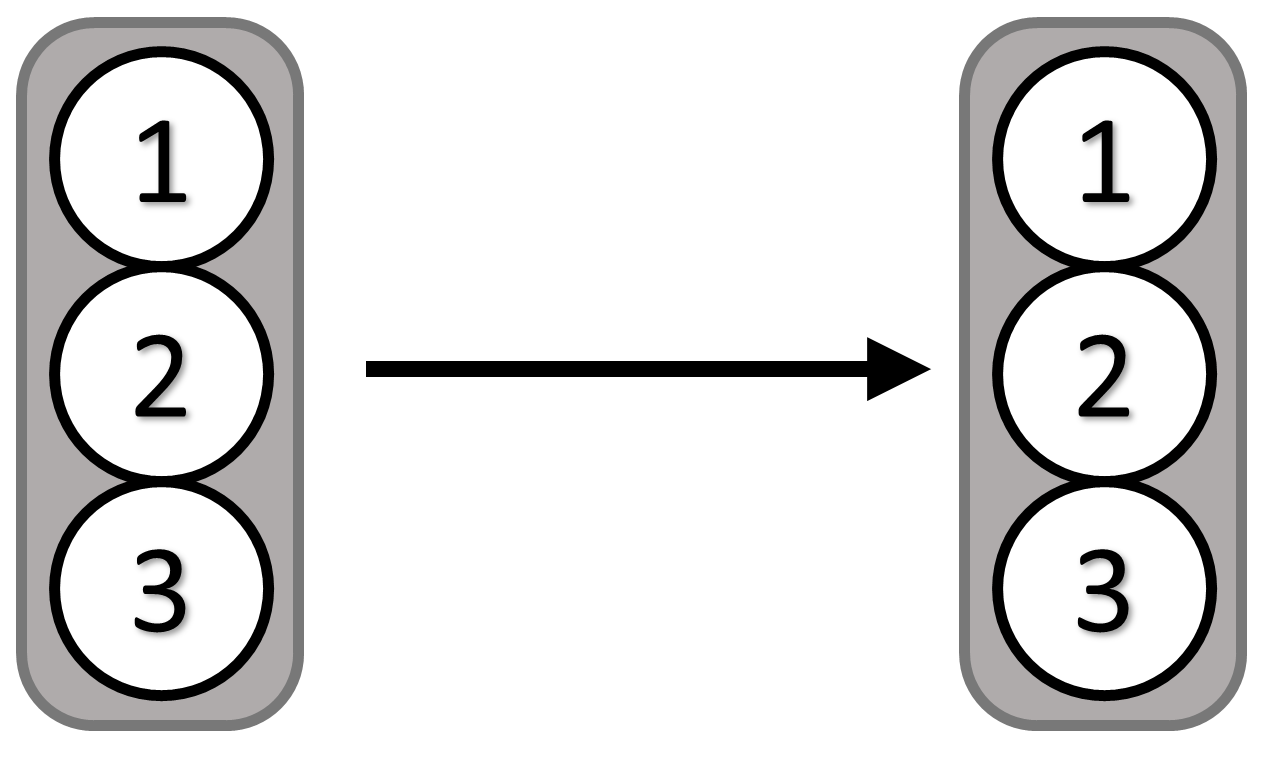
\includegraphics[scale=0.85]{EMU_reaction_3.png}
			 	\end{minipage}
			 } 
		     & \adj{$C_{123} = A_{123}$}\\[.5ex]
				& \adj{$C_{123,M+0} = A_{123,M+0}$}\\ [.5ex]
				& \adj{$C_{123,M+1} = A_{123,M+1}$}\\ [.5ex]
				& \adj{$C_{123,M+2} = A_{123,M+2}$} \\ [.5ex]
				& \adj{$C_{123,M+3} = A_{123,M+3}$} \\ [.5ex]
			 \hline 
		\end{tabular}
		\caption{EMU-реакции}
		\label{EMU_reactions}
	\end{center}
\end{table} % ---------------------- Можно что-то вписать
\begin{figure}[h!]
	\centering
	\begin{minipage}[l]{.5\textwidth}
		\centering
		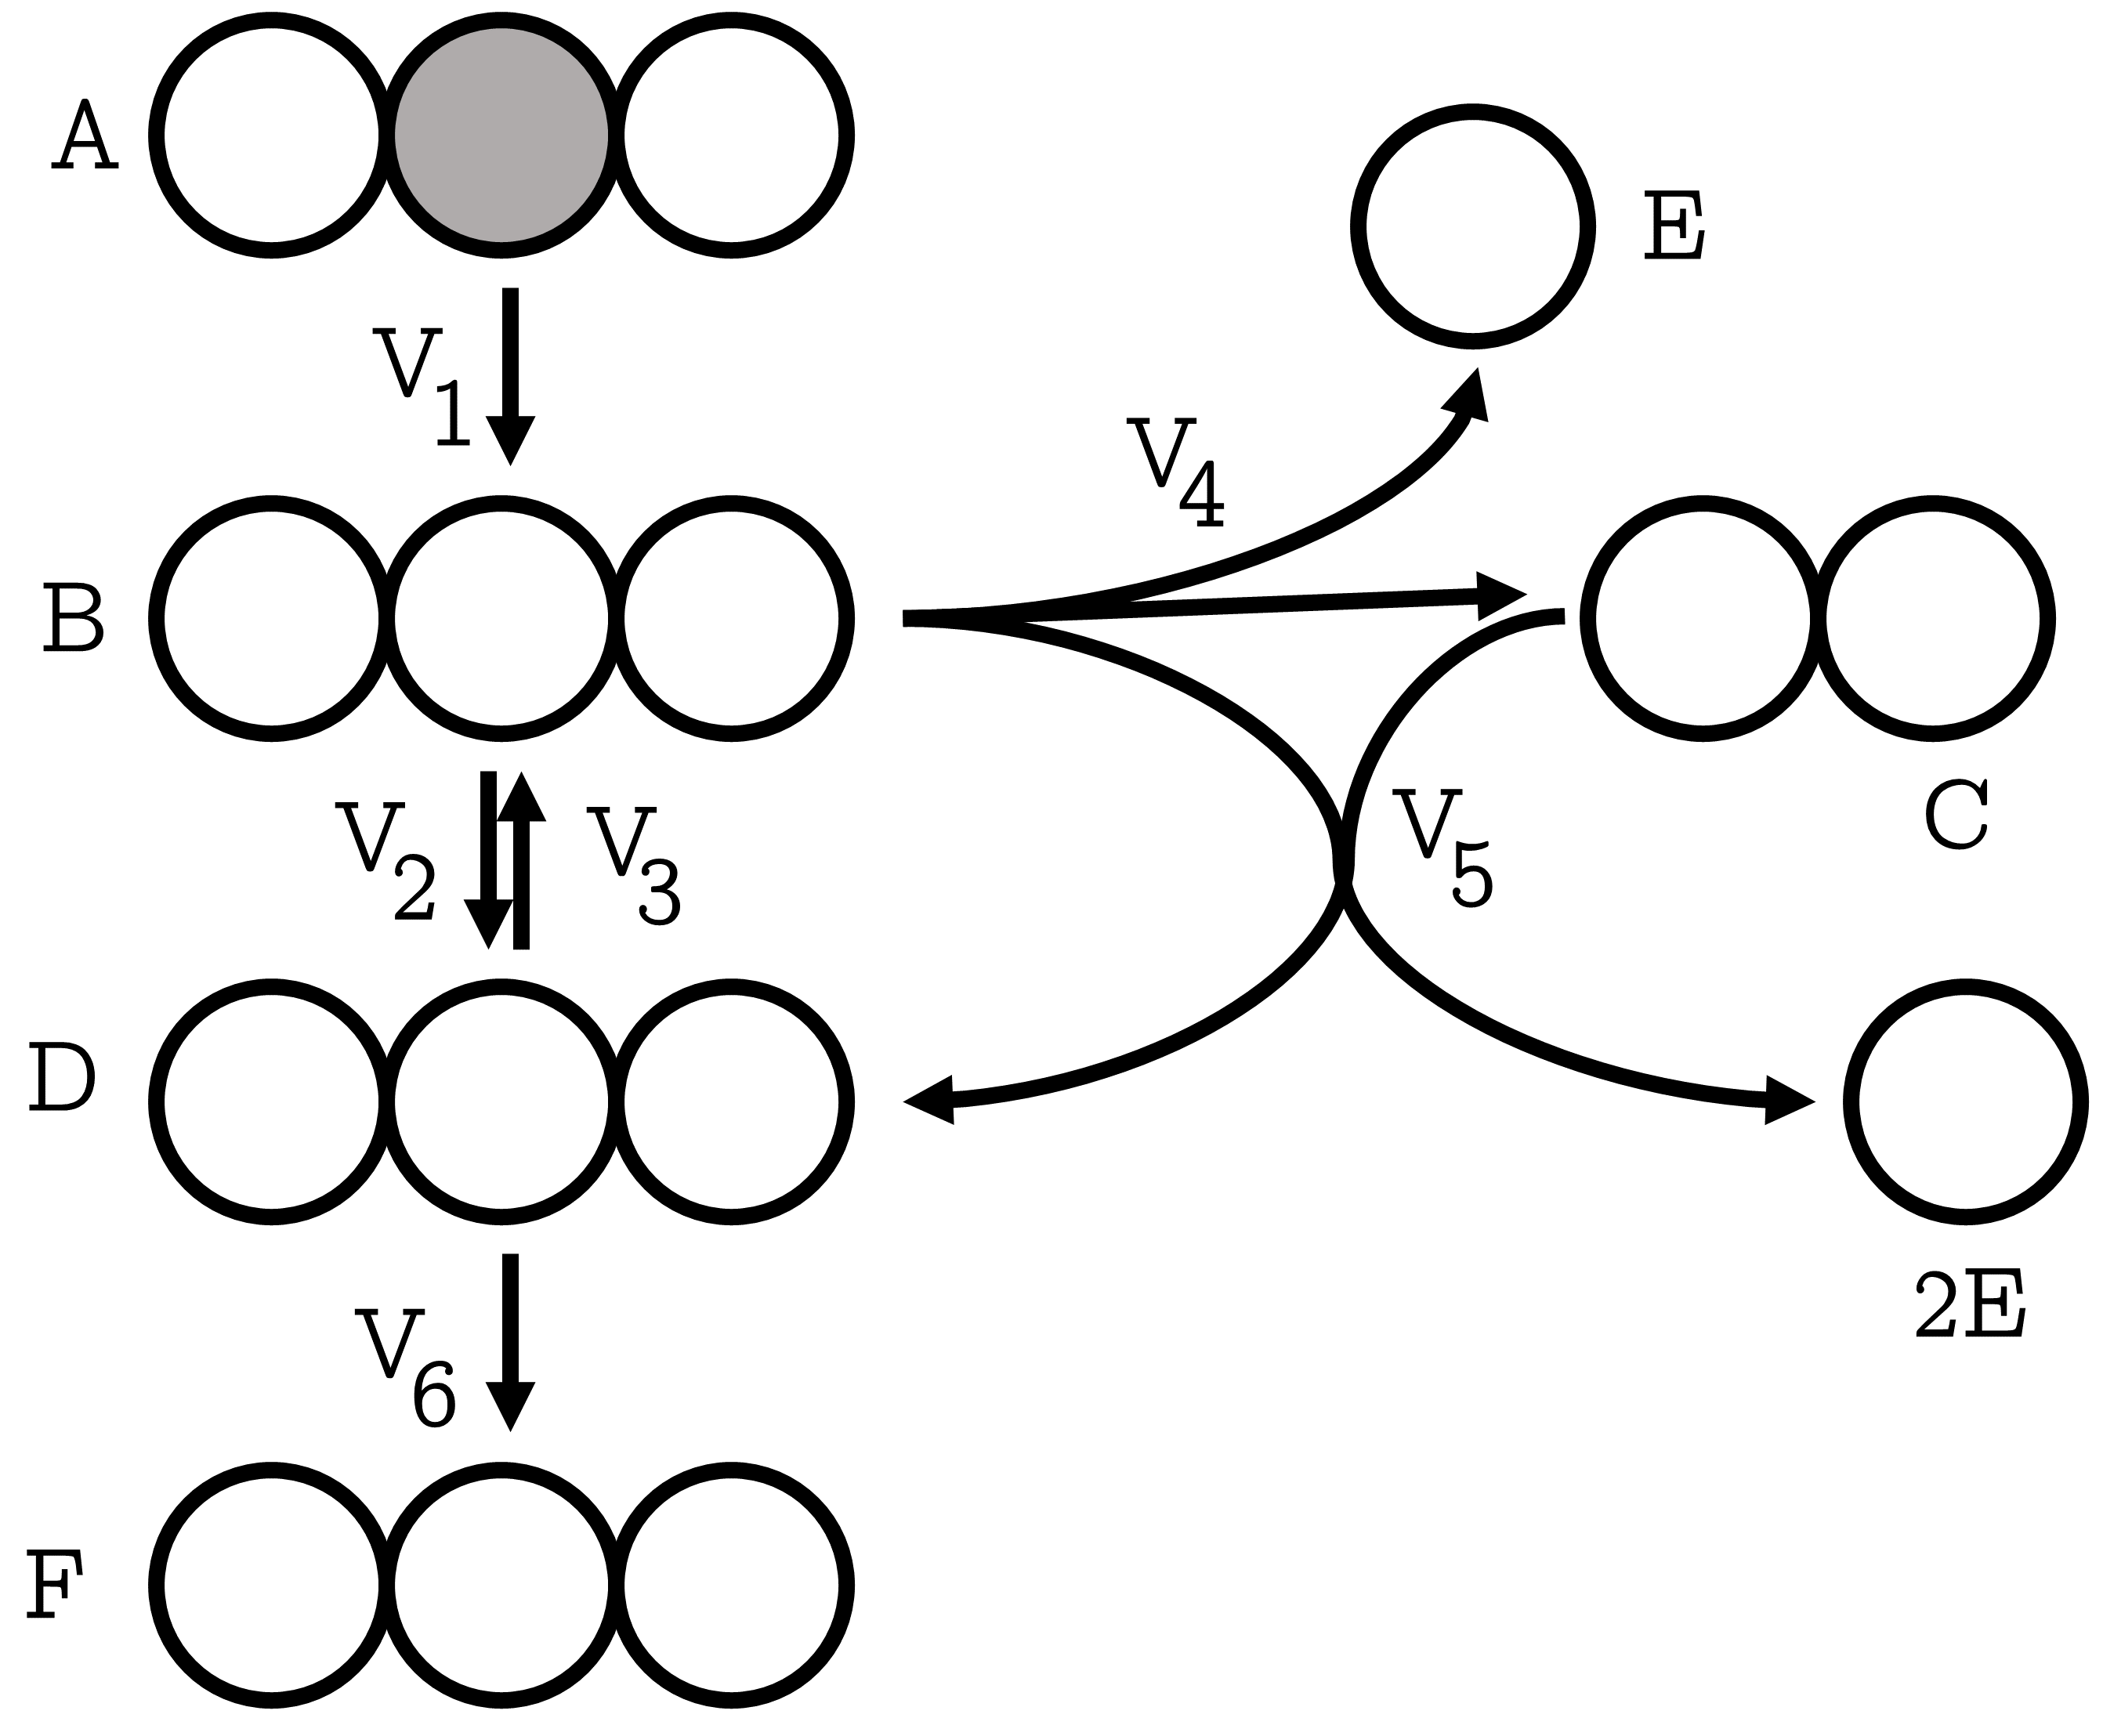
\includegraphics[scale=0.11]{full_emu_map.png}
		\caption{Метаболическая сеть}
		\label{emu_example}
	\end{minipage}%
	\begin{minipage}[r]{.5\textwidth}
		\centering
		\small
		\begin{tabular}{c c c}
			\hline
			№ & Реакция & Переходы трейсера\\
			\hline
			1 & $A \to B$ & abc $\leftrightarrow$ abc\\
			2 и 3 & B $\leftrightarrow$ D & abc $\leftrightarrow$ abc\\
			4 & B $\to$ C + E & abc $\to$bc + a\\
			5 & B+C $\to$ D+E+E & abc+de $\to$ bcd+a+e\\
			6 & D $\to$ F & abc $\to$ abc\\
			\hline
		\end{tabular}
		\captionof{table}{Ее химические уравнения}
		\label{emu_example_table}
	\end{minipage}
\end{figure}


\clearpage
\begin{wraptable}[25]{l}{0.5\linewidth}
	\begin{tabular}{c c c}
		\hline
		№ & EMU-реакция & Размер\\
		\hline
		6 & $D_{123} \to F_{123}$ & $3 = 3$\\
		2 & $B_{123} \to D_{123}$ & $3 = 3$\\
		5 & $B_{23} + C_1 \to D_{123}$ & $2 + 1 = 3$\\
		1 & $A_{123} \to B_{123}$ & $3 = 3$\\
		3 & $D_{123} \to B_{123}$ & $3 = 3$\\
		1 & $A_{23} \to B_{23}$ & $2 = 2$\\
		3 & $D_{23} \to B_{23}$ & $2 = 2$\\
		2 & $B_{23} \to D_{23}$ & $2 = 2$\\
		5 & $B_3 + C_1 \to D_{23}$ & $1 + 1 = 2$\\
		4 & $B_2 \to C_1$ & $1 = 1$\\
		1 & $A_2 \to B_2$ & $1 = 1$\\
		3 & $D_2 \to B_2$ & $1 = 1$\\
		2 & $B_2 \to D_2$ & $1 = 1$\\
		5 & $B_3 \to D_2$ & $1 = 1$\\
		1 & $A_3 \to B_3$ & $1 = 1$\\
		3 & $D_3 \to B_3$ & $1 = 1$\\
		2 & $B_3 \to D_3$ & $1 = 1$\\
		5 & $C_1 \to D_3$ & $1 = 1$\\
	\end{tabular}
	\caption{Список реакций, для определения MID $F_{123}$}
	\label{all_emu_reactions}
\end{wraptable}


Рассмотрим пример. Пусть дана метаболическая сеть с рис. \ref{emu_example}. Известна меченность входного субстрата $A$, то есть известны MID всех EMU $A$. Требуется найти $F_{123}$. Оно формируется в EMU-реакции $$D_{123} \to F_{123}$$ поэтому надо узнать $D_{123}$. Оно задается двумя EMU-реакциями: $$B_{123} \leftrightarrow D_{123}$$ $$B_{23} + C_1 \to D_{123}$$Теперь надо определить $B_{123}$, $B_{23}$ и $C_1$. Проведя поиск в глубину, найдем список EMU, MID которых надо узнать и заодно составим список EMU-реакций. Реакции нашего примера выписаны в таблице \ref{all_emu_reactions}.

Для всех EMU-реакций одного размера построим EMU-граф. Это ориентированный граф, вершины которого --- субстраты и продукты EMU-реакций, причем субстратам реакций конденсации сопоставим свертки, согласно таблице \ref{EMU_reactions}. Например, $B_{23} + C_1 = B_{23} \times C_1$. Обратим внимание, что вершины, не имеющие входящих ребер, либо являются входными EMU, чьи MID известны, либо являются сверткой EMU меньшего размера. EMU-графы нашего примера на рис. \ref{emu_graph}.

\begin{figure}[b]
	\begin{subfigure}{.3\linewidth}
		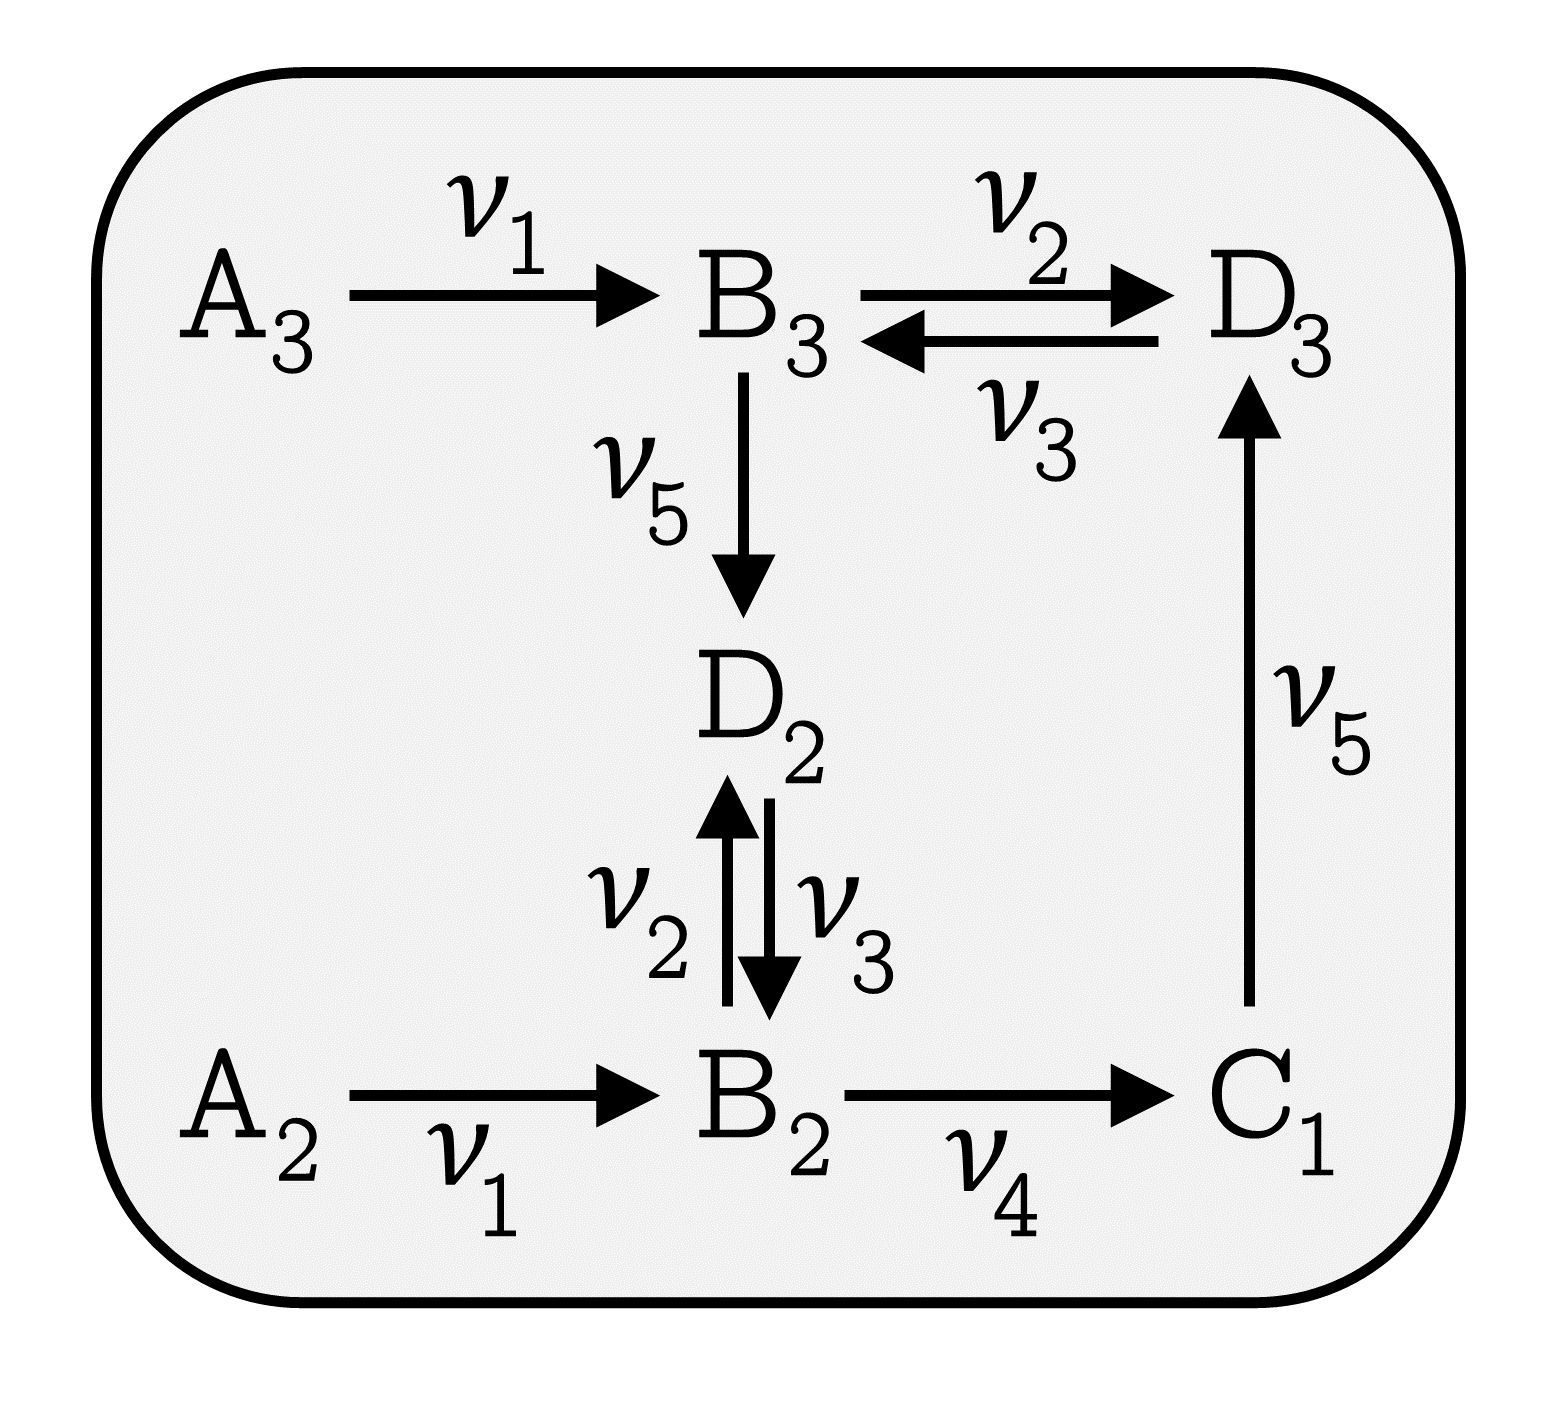
\includegraphics[width=\linewidth]{EMU_graph_1.png}
		\caption{размера 1}
		\label {emu_graph_1}
	\end{subfigure}
	\begin{subfigure}{.3\linewidth}
		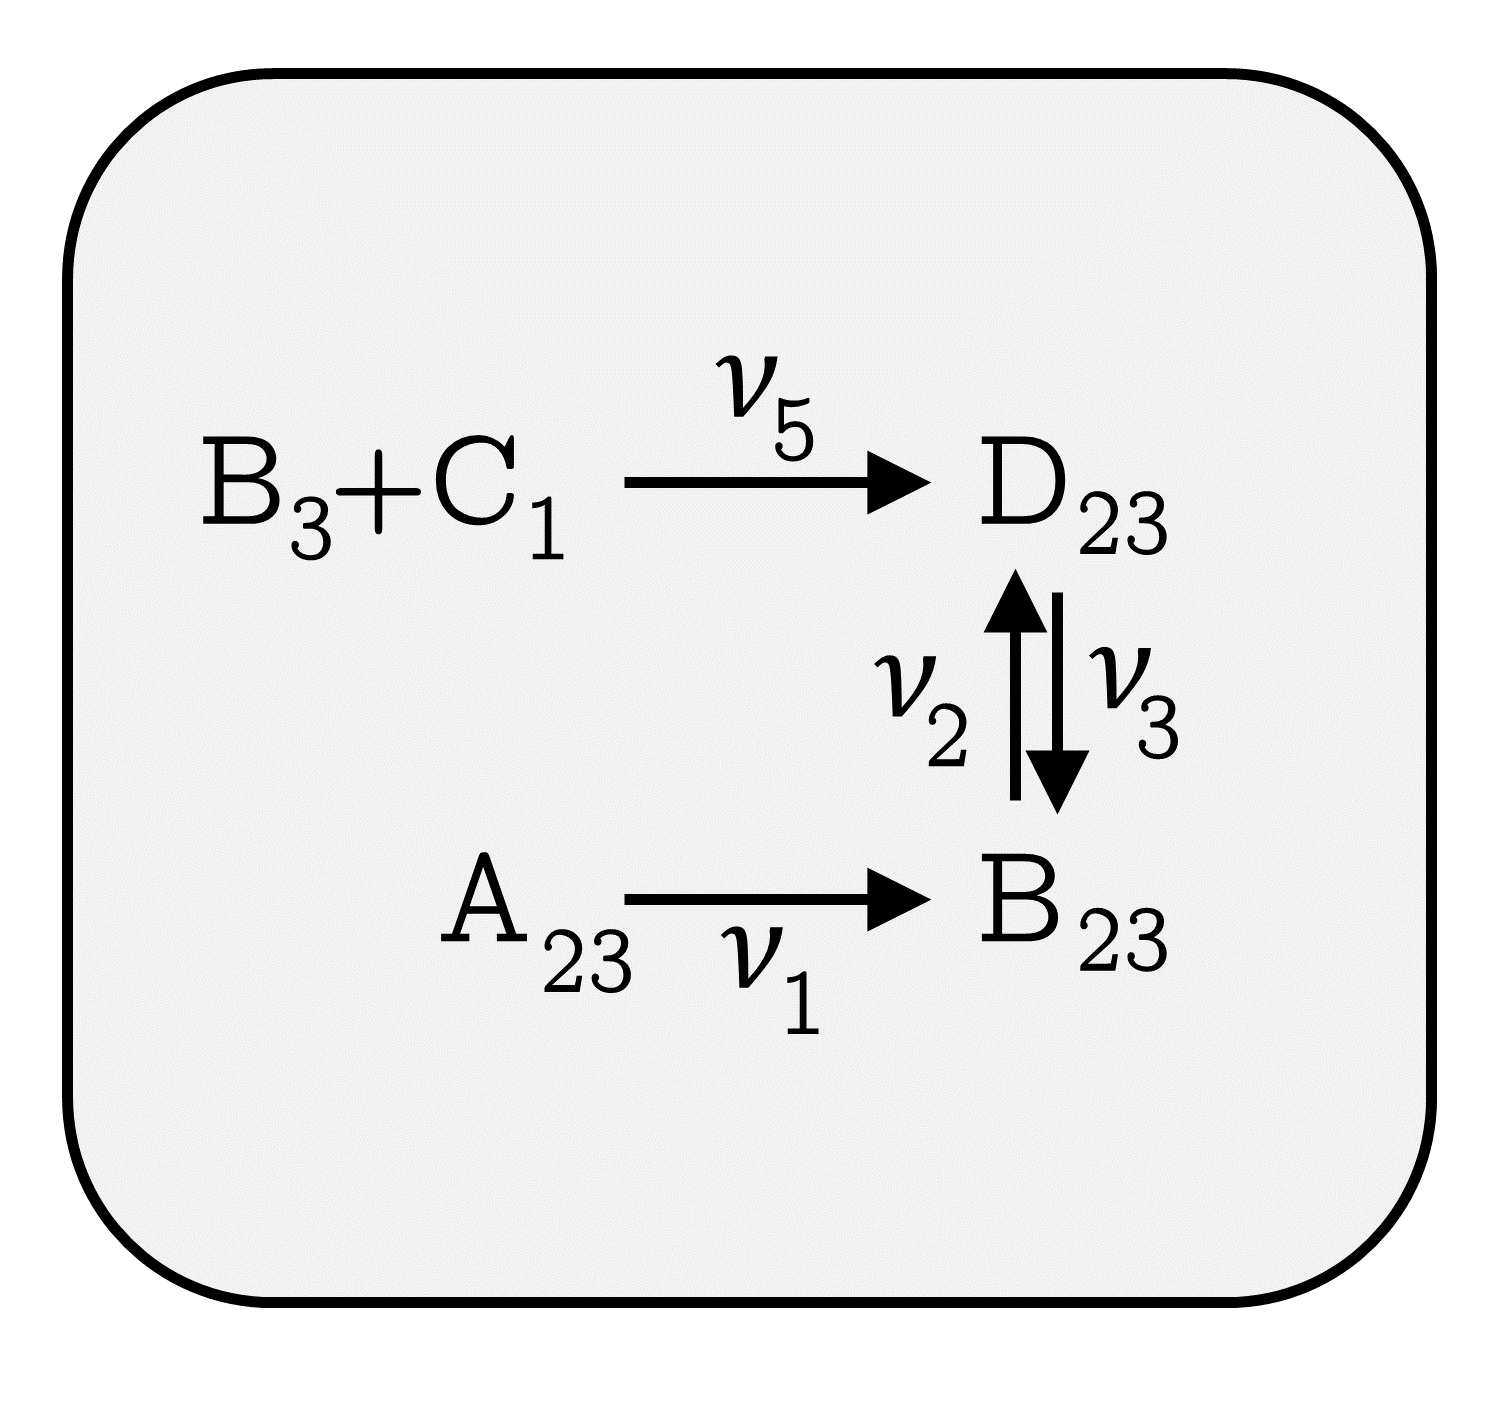
\includegraphics[width=\linewidth]{EMU_graph_2.png}
		\caption{размера 2}
		\label {emu_graph_2}
	\end{subfigure}
	\begin{subfigure}{.3\linewidth}
		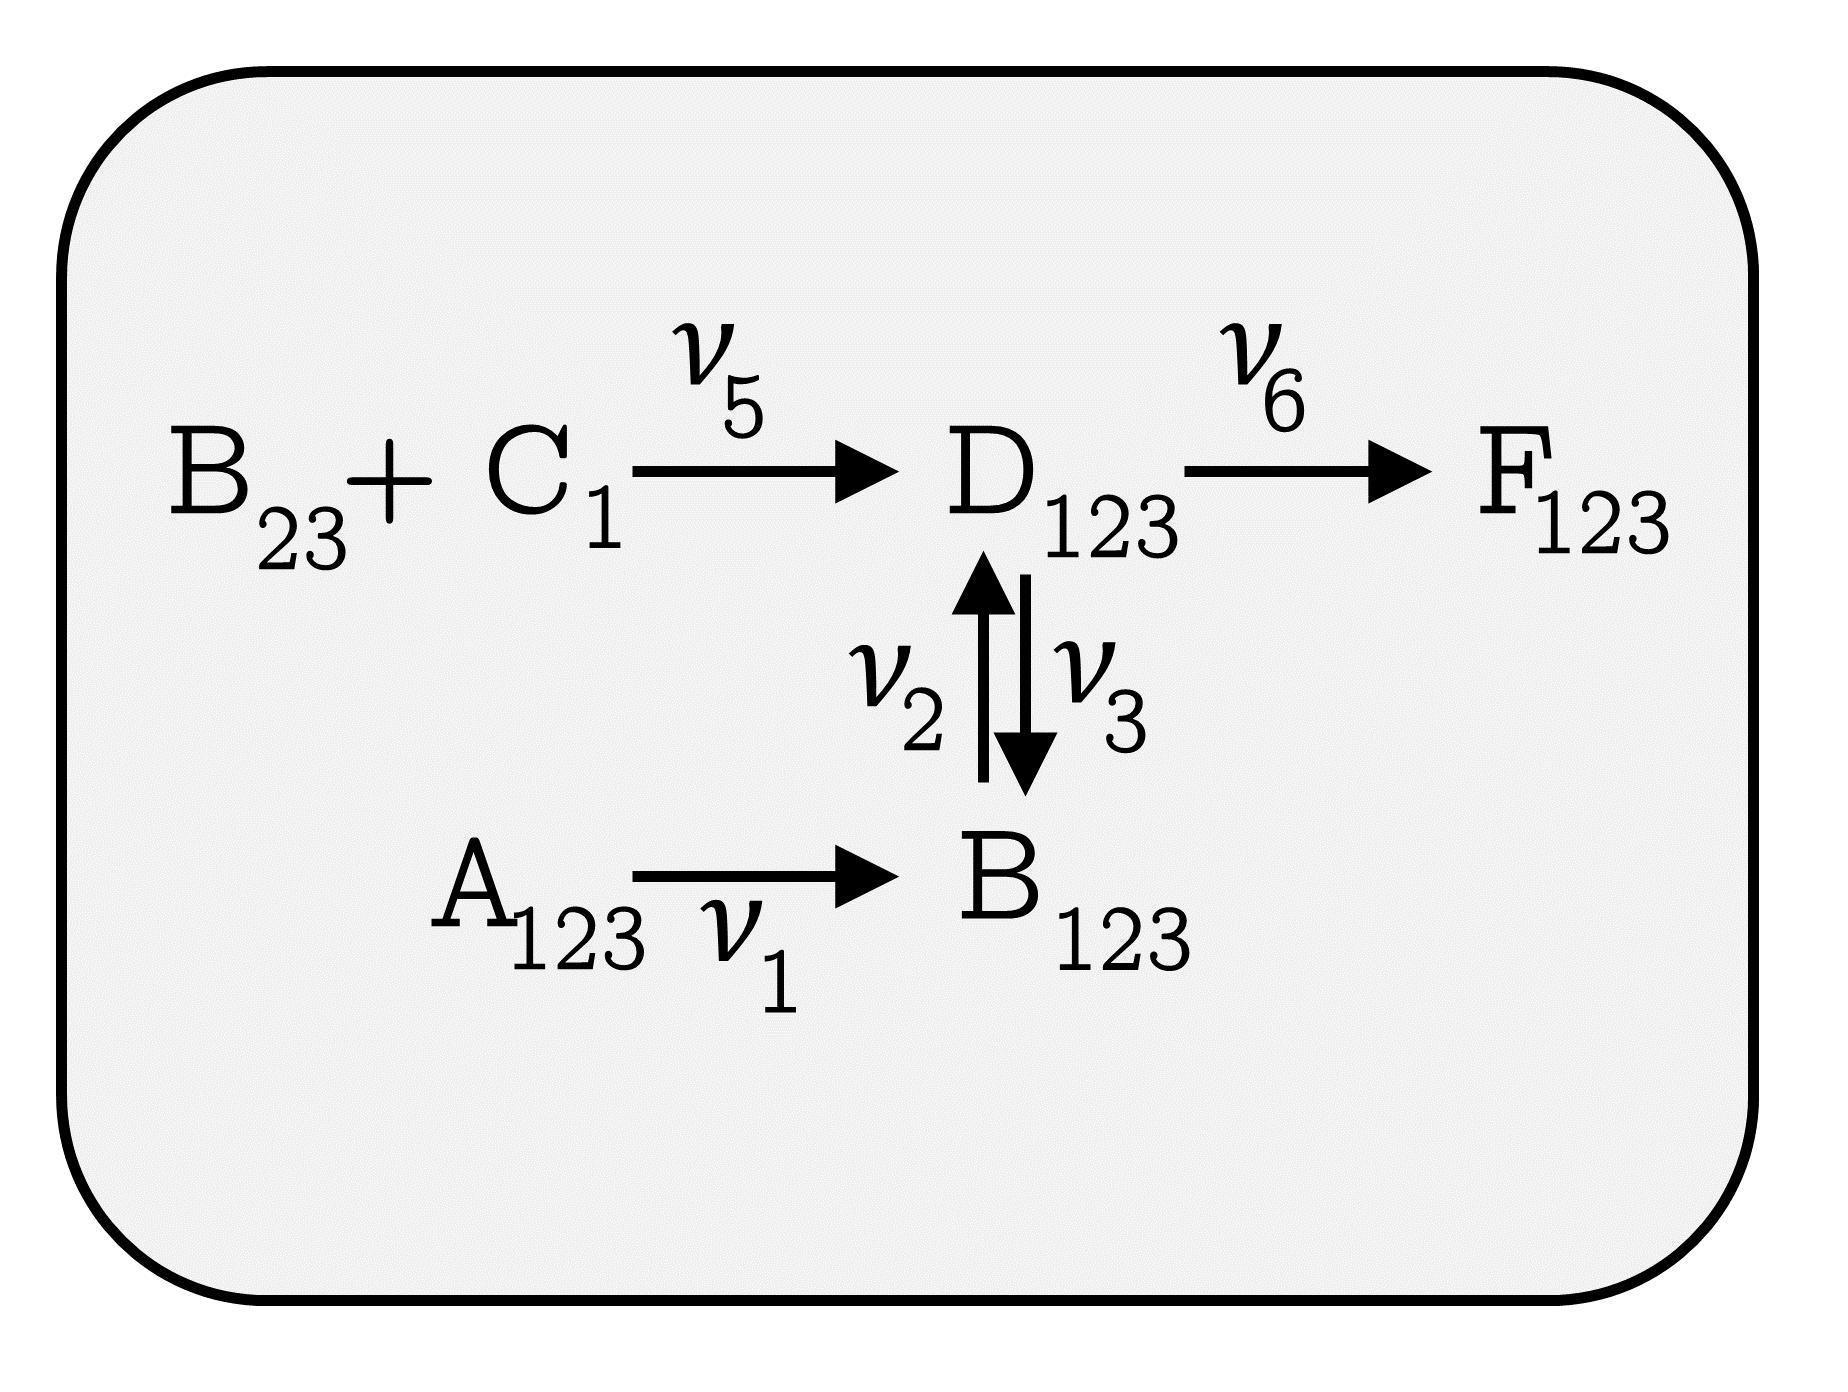
\includegraphics[width=1.2\linewidth]{EMU_graph_3.png}
		\caption{размера 3}
		\label {emu_graph_3}
	\end{subfigure}
	\caption{EMU-графы}
	\label{emu_graph}
\end{figure}

\clearpage

\subsection{Каскад уравнений}
Для каждого EMU-графа составим СЛАУ:
$$A(v)X = B(v)Y$$
Строки $X$ --- это неизвестные MID графа.

\noindent $A(v)$ --- матрица потоков такая, что 
$a_{ij} = 
\begin{cases} 
	\text{$-\sum$потоков исходящих из $X_i$, $i=j$}\\
	\text{поток из $X_i$ в $X_j$, $i\neq{}j$}
	\end{cases}
	$
Матрица $Y$ содержит известные MID, так что $y_{ij}$ равняется массовой доле молекул $i$-го EMU с известным MID с $j - 1$ атомами трейсера. $B(v)$ составляется аналогично $A$.
Известно, что при ненулевых потоках, матрицы $A(v)$ обратимы\cite{anderson_1983}. Найдя $X = A^{-1}B(v)Y$, мы найдем MID всех EMU графа. Часть из них используется для решения СЛАУ следующего уровня.

Таким образом получим каскад СЛАУ:
$$A_1(v)X_1 = B_1(v)Y_1(x_{in})$$
$$A_2(v)X_2 = B_2(v)Y_2(x_{in}, X_1)$$
$$\dots$$
$$A_n(v)X_n = B_n(v)Y_n(x_{in}, X_1, \ldots, X_{n - 1})$$
Решив его, найдем искомые MID. В нашем примере уравнения выглядят так:

$$\begin{bmatrix}
-v_4 & v_4 & 0 & 0 & 0\\
0 & -v_1-v_3 & v_3 & 0 & 0\\
0 & v_2 & -v_2-v_5 & v_5 & 0\\
0 & 0 & 0 & -v_1-v_3 & v_3 \\
v_5 & 0 & 0 & v_2 & -v_2-v_5\\
\end{bmatrix}
\begin{bmatrix}
	C_1\\
	B_2\\
	D_2\\
	B_3\\
	D_3\\
\end{bmatrix}
=
\begin{bmatrix}
	0 & 0\\
	-v_1 & 0\\
	0 & 0\\
	0 & -v_1\\
	0 & 0\\
\end{bmatrix}
\begin{bmatrix}
	A_2\\
	A_3\\
\end{bmatrix}$$

$$\begin{bmatrix}
-v_5-v_2 & v_2\\
v_3 & -v_1-v_3\\
\end{bmatrix}
\begin{bmatrix}
D_{23}\\
B_{23}
\end{bmatrix}
=
\begin{bmatrix}
-v_5 & 0\\
0 & -v_1\\
\end{bmatrix}
\begin{bmatrix}
B_3 \times C_1\\
A_{23}
\end{bmatrix}$$

$$\begin{bmatrix}
-v_6 & v_6 & 0\\
0 & -v_5-v_2 & v_2\\
0 & v_3 & -v_1-v_3\\
\end{bmatrix}
\begin{bmatrix}
F_{123}\\
D_{123}\\
B_{123}\\
\end{bmatrix}
=
\begin{bmatrix}
0 & 0\\
-v_5 & 0\\
0 & -v_1\\
\end{bmatrix}
\begin{bmatrix}
B_{23} \times C_1\\
A_{123}\\
\end{bmatrix}
$$
\clearpage
\section{Статистический анализ}
\subsection{Статистическая значимость}
Результаты решения регрессии надо проверить на статистическую\\ значимость\cite{shupltesov_review_2}. Будем считать, что каждый член суммы формулы (1.1) является случайной величиной $\sim \mathcal{N}(0, 1)$. Гипотеза $H_0$ заключается в том, что сумма квадратов разностей $\xi_{SSR}$ (1.1), являясь суммой случайных величин, удовлетворяет распределению $\chi^2$. Число степеней свободы этого распределения равно числу независимых измерений $W$ минус число оцениваемых параметров (то есть число свободных потоков) $p$. $H_1$ --- значит, что $\xi_{SSR}$ имеет другое распределение. Таким образом, критерий значимости:
$$
\sigma(\xi_{SSR}) = \begin{cases}
	H_0,&\text{если $\chi^2_{\alpha / 2}(W - p) \le \xi_{SSR} \le \chi^2_{1 - \alpha}(W - p)$}\\
	H_0,&\text{если $\xi_{SSR} \leq \chi^2_{\alpha / 2}(W - p)$, но возможна переподгонка}\\
	H_1,&\text{если $\xi_{SSR} \geq \chi^2_{1 - \alpha}(W - p)$}\\
\end{cases}$$
\subsection{Доверительные интервалы}

\chapter[Постановка задачи]{\thechapter{}. Постановка задачи}
\begin{itemize}
	\item Написать программу для расчета \ce{^{13}C}-MFA на языке \CC.
	\item Провести тестирование, сравнить скорость работы с существующими аналогами.
\end{itemize}

\chapter[Основная часть]{\thechapter{}. Основная часть}
\section{Программа Khnum}
Программа написана так-то. В ней то-то. 

\section{Тестирование}
Так убедился в корректности.

\subsection{Корректность}

\subsection{Производительность}
Во как быстро.

\chapter[Полученные результаты]{\thechapter{}. Полученные результаты}
Кратко: написано, протестировано, замерено.

\chapter[Заключение]{\thechapter{}. Заключение}
Было сделано. 
\section{Дальнейшая работа}
Попробую вот это.


\begin{appendices}
	\chapter{Список программ для MFA-расчетов}
	\begin{itemize}
		\item \textbf{13CFLUX2} --- Самая известная программа для \ce{^{13}C}-MFA. Имеет закрытый исходный код и платна для коммерческого использования. Для научных целей можно получить академическую лицензию, написав письмо в Германию\cite{13CFLUX2}.
		
		\item \textbf{Metran} --- Написана автором EMU-модели. Чтобы получить программу под академической лицензией надо написать письмо в MIT\cite{Metran}.
		
		\item \textbf{OpenFlux(2)} --- Пакет для Matlab\cite{OpenFlux, OpenFlux2}.
		
		\item \textbf{FluxPyt} --- Пакет для Python\cite{FluxPyt}.
	\end{itemize}
	
	
	\chapter{Формальное определение \\метаболической сети}
	Пусть $V$ -- конечное множество \emph{метаболитов}. Для каждого метаболита известно \emph{число атомов трейсера} в нем: $\mathbb{C} \colon V \to \mathbb{N}_0$. 
	
	Пусть $U, W \subset V$ --- конечные мультимножества метаболитов. \emph{Химической реакцией} назовем упорядоченную пару $e = (U, W)$, элементы которой назовем \emph{субстратом} и \emph{продуктом} соответственно, если:
	\begin{itemize}
		\item Количество атомов трейсера одинаково в субстрате и продукте: \\ $n = \sum_{u \in U} \mathbb{C}(u) = \sum_{w \in W} \mathbb{C}(w_j)$. 
		\item Задана перестановка $S_e$ с мощностью, равной количеству атомов трейсера в субстрате и продукте $|S_e| = n$.
	\end{itemize}
	
	\emph{Метаболической сетью} будем называть ориентированный гиперграф $G = (V, E)$, такой что каждое ребро $e \in E$ является химической реакцией.
\end{appendices}

\cleardoublepage
\phantomsection
\addcontentsline{toc}{chapter}{Список литературы}
\renewcommand{\bibname}{Список литературы}
\begin{thebibliography}{XXXX}
	\bibitem{Cancer_statistics}
	Всемирная Ассоциация Здравоохранения. Cancer [Электронный ресурс] URL: https://www.who.int/news-room/fact-sheets/detail/cancer (дата обращения: 12.03.2020)
	
	\bibitem{Warburg_effect}
	Warburg O., Wind F., Negelein E. The metabolism of tumors in the body // The Journal of general physiology.--- 1927. --- Т. 8. --- №. 6. --- С. 519.
	
	\bibitem{Diabetes_statistics}
	Zimmet P. et al. Diabetes mellitus statistics on prevalence and mortality: facts and fallacies Nature Reviews Endocrinology. --- 2016. --- Т. 12. --- №. 10. --- С. 616.
	
	\bibitem{Genentech_paper}
	Cohen S. N. et al. Construction of biologically functional bacterial plasmids in vitro // Proceedings of the National Academy of Sciences. --- 1973. --- Т. 70. --- №. 11. --- С. 3240--3244.
	
	\bibitem{Application_cancer_2009}
	Metallo C. M., Walther J. L., Stephanopoulos G. Evaluation of 13C isotopic tracers for metabolic flux analysis in mammalian cells // Journal of biotechnology. --- 2009. --- Т. 144. --- №. 3. --- С. 167--174.
	
	\bibitem{Application_cancer_2012}
	Walther J. L. et al. Optimization of 13C isotopic tracers for metabolic flux analysis in mammalian cells // Metabolic engineering. --- 2012. --- Т. 14. --- №. 2. --- С. 162--171.
	
	\bibitem{Application_cancer_2013}
	Hiller K., Metallo C. M. Profiling metabolic networks to study cancer metabolism // Current opinion in biotechnology. --- 2013. --- Т. 24. --- №. 1. --- С. 60--68.
	
	\bibitem{Application_cancer_2015}
	Boroughs L. K., DeBerardinis R. J. Metabolic pathways promoting cancer cell survival and growth // Nature cell biology. --- 2015. --- Т. 17. --- №. 4. --- С. 351--359.
	
	\bibitem{Application_cancer_2017}
	Dong W., Keibler M. A., Stephanopoulos G. Review of metabolic pathways activated in cancer cells as determined through isotopic labeling and network analysis // Metabolic engineering. --- 2017. --- Т. 43. --- С. 113--124.
	
	\bibitem{Application_cancer_2018}
	Antoniewicz M. R. A guide to 13 C metabolic flux analysis for the cancer biologist // Experimental \& molecular medicine. --- 2018. --- Т. 50. --- №. 4. --- С. 1--13.
	
	\bibitem{Application_cancer_2018_2}
	Badur M. G., Metallo C. M. Reverse engineering the cancer metabolic network using flux analysis to understand drivers of human disease // Metabolic engineering. --- 2018. --- Т. 45. --- С. 95--108.
	
	\bibitem{Application_engeneering_2009}
	Nakahigashi K. et al. Systematic phenome analysis of Escherichia coli multiple‐knockout mutants reveals hidden reactions in central carbon metabolism // Molecular systems biology. --- 2009. --- Т. 5. --- №. 1.
	
	\bibitem{Application_engeneering_2015}
	Crown S. B., Long C. P., Antoniewicz M. R. Integrated 13C-metabolic flux analysis of 14 parallel labeling experiments in Escherichia coli // Metabolic engineering. --- 2015. --- Т. 28. --- С. 151--158.
	
	\bibitem{Application_engeneering_2017}
	Long C. P. et al. Enzyme I facilitates reverse flux from pyruvate to phosphoenolpyruvate in Escherichia coli // Nature communications. --- 2017. --- Т. 8. --- №. 1. --- С. 1--8.
	
	\bibitem{Application_other_2011}
	Wahrheit J., Nicolae A., Heinzle E. Eukaryotic metabolism: measuring compartment fluxes // Biotechnology journal. --- 2011. --- Т. 6. --- №. 9. --- С. 1071--1085.
	
	\bibitem{Application_other_2013}
	Metallo C. M., Vander Heiden M. G. Understanding metabolic regulation and its influence on cell physiology // Molecular cell. --- 2013. --- Т. 49. --- №. 3. --- С. 388--398.
	
	\bibitem{Application_other_2014}
	Dieuaide-Noubhani M., Alonso A. P. (ed.). Plant metabolic flux analysis: methods and protocols. --- Humana Press, 2014.
	
	\bibitem{nitrogen_mfa}
	Nilsson R., Jain M. Simultaneous tracing of carbon and nitrogen isotopes in human cells // Molecular BioSystems. --- 2016. --- Т. 12. --- №. 6. --- С. 1929--1937.
	
	\bibitem{sulfur_mfa}
	Krömer J. O. et al. Accumulation of homolanthionine and activation of a novel pathway for isoleucine biosynthesis in Corynebacterium glutamicum McbR deletion strains // Journal of bacteriology. --- 2006. --- Т. 188. --- №. 2. --- С. 609--618.
	
	\bibitem{protocol}
	Systems Metabolic Engineering. Methods and Protocols. // Под ред. Alper, Hal S. --- 1 изд. Humana Press, 2013. --- 474 с.
	
	\bibitem{protocol_animal}
	(ed.). Metabolic flux analysis: methods and protocols. // Под ред. Krömer J. O., Nielsen L. K., Blank L. M. --- 1 изд. Humana Press, 2014. --- 329 с.
	
	\bibitem{protocol_plant}
	Plant metabolic flux analysis: methods and protocols. // Под ред. Dieuaide-Noubhani M., Alonso A.P. --- 1 изд. Humana Press, 2014. --- 366 с.
	
	\bibitem{first_MFA}
	Blumstein S. E., Isaacs E., Mertus J. The role of the gross spectral shape as a perceptual cue to place of articulation in initial stop consonants // The Journal of the Acoustical Society of America. – 1982. – Т. 72. – №. 1. – С. 43-50.
	
	\bibitem{Wiechert_1997_1}
	Wiechert W., de Graaf A. A. Bidirectional reaction steps in metabolic networks: I. Modeling and simulation of carbon isotope labeling experiments // Biotechnology and bioengineering. --- 1997. --- Т. 55. --- №. 1. --- С. 101--117.
	
	\bibitem{Wiechert_1997_2}
	Wiechert W. et al. Bidirectional reaction steps in metabolic networks: II. Flux estimation and statistical analysis // Biotechnology and bioengineering. --- 1997. --- Т. 55. --- №. 1. --- С. 118--135.
	
	\bibitem{Wiechert_1999_3}
	Wiechert W. et al. Bidirectional reaction steps in metabolic networks: III. Explicit solution and analysis of isotopomer labeling systems // Biotechnology and bioengineering. --- 1999. --- Т. 66. --- №. 2. --- С. 69--85.
	
	\bibitem{Wiechert_1999_4}
	Möllney M. et al. Bidirectional reaction steps in metabolic networks: IV. Optimal design of isotopomer labeling experiments // Biotechnology and bioengineering. --- 1999. --- Т. 66. --- №. 2. --- С. 86---103.
	
	\bibitem{13CFlux1}
	Wiechert W. et al. A universal framework for 13C metabolic flux analysis // Metabolic engineering. --- 2001. --- Т. 3. --- №. 3. --- С. 265-283.
	
	\bibitem{Direct_MFA}
	Rantanen A. et al. Algorithms for 13C metabolic flux analysis. --- 2006.
	
	\bibitem{Markov_chain_MFA}
	Huo Y., Ji P. Continuous-Time Markov Chain–Based Flux Analysis in Metabolism // Journal of Computational Biology. --- 2014. --- Т. 21. --- №. 9. --- С. 691-698.
	
	\bibitem{Fluxomer_MFA}
	Srour O., Young J. D., Eldar Y. C. Fluxomers: a new approach for 13 C metabolic flux analysis // BMC systems biology. --- 2011. --- Т. 5. --- №. 1. --- С. 129.
		
	\bibitem{13CFLUX2}
	Weitzel M. et al. 13CFLUX2—high-performance software suite for 13C-metabolic flux analysis // Bioinformatics. --- 2013. --- Т. 29. --- №. 1. --- С. 143--145.
	
	\bibitem{Metran}
	Yoo H. et al. Quantifying reductive carboxylation flux of glutamine to lipid in a brown adipocyte cell line // Journal of Biological Chemistry. --- 2008 --- Т. 283. --- №. 30. --- С. 20621-20627.
	
	\bibitem{OpenFlux}
	Quek L. E. et al. OpenFLUX: efficient modelling software for 13 C-based metabolic flux analysis // Microbial cell factories. --- 2009. --- Т. 8. --- №. 1. --- С. 25.
	
	\bibitem{OpenFlux2}
	Shupletsov M. S. et al. OpenFLUX2: 13 C-MFA modeling software package adjusted for the comprehensive analysis of single and parallel labeling experiments // Microbial cell factories. --- 2014. --- Т. 13. --- №. 1. --- С. 152.
	
	\bibitem{FluxPyt}
	Desai T. S., Srivastava S. FluxPyt: a Python-based free and open-source software for 13C-metabolic flux analyses // PeerJ. --- 2018. --- Т. 6. --- С. e4716.
	
	\bibitem{NMFA}
	Wiechert W., Nöh K. Isotopically non-stationary metabolic flux analysis: complex yet highly informative // Current opinion in biotechnology. --- 2013. --- Т. 24. --- №. 6. --- С. 979--986.
	
	\bibitem{DMFA}
	Leighty R. W., Antoniewicz M. R. Dynamic metabolic flux analysis (DMFA): a framework for determining fluxes at metabolic non-steady state // Metabolic engineering. --- 2011. --- Т. 13. --- №. 6. --- С. 745--755.

	\bibitem{formalizm_2017}
	Borkum M. I. et al. Modeling framework for isotopic labeling of heteronuclear moieties // Journal of cheminformatics. --- 2017. --- Т. 9. --- №. 1. --- С. 1--11.
	
	\bibitem{EMU_2007}
	Antoniewicz M. R., Kelleher J. K., Stephanopoulos G. Elementary metabolite units (EMU): a novel framework for modeling isotopic distributions // Metabolic engineering. --- 2007 --- Т. 9. --- №. 1. --- С. 68--86.
	
	\bibitem{shupltesov_review_2}
	Шуплецов М. С., Голубева Л. И., Машко С. В. Анализ метаболических потоков с использованием 13 С-изотопов (13 C-MFA). II. Математические основы метода // Биотехнология --- 2016. --- Т. 32. --- №. 6. --- С. 9-34.
	
	\bibitem{anderson_1983}
	Anderson M. J., Fambrough D. M. Aggregates of acetylcholine receptors are associated with plaques of a basal lamina heparan sulfate proteoglycan on the surface of skeletal muscle fibers // The Journal of cell biology. --- 1983. --- Т. 97. --- №. 5. --- С. 1396-1411.
	
	
\end{thebibliography}



\end{document}          
